\section{Details of Experiments}


% % % % % % % % % % % % % % % % % % % % % % % % % % % % % %
\subsection{Experimental Environments and Implementation Information} \label{app:implementation}
% % % % % % % % % % % % % % % % % % % % % % % % % % % % % %

We used the following computers for experiments:
For experiments except for the image dataset,
we run experiments on a computer with Intel Xeon Silver 4214R (2.40GHz) CPU and 64GB RAM.
For experiments using the image dataset,
we run experiments on a computer with Intel(R) Xeon(R) Gold 6338 (2.00GHz) CPU, NVIDIA RTX A6000 GPU and 1TB RAM.

Procedures are implemented in Python, mainly with the following libraries:
\begin{itemize}
\item {\em NumPy} \citep{harris2020array}: Matrix and vector operations
\item {\em CVXPY} \citep{diamond2016cvxpy}: Convex optimizations (training computations with weights)
\item {\em SciPy} \citep{2020SciPy-NMeth}: Solving equations to maximize the quadratic convex function in \eqref{eq:maximum-gap} (by module {\em optimize.root\_scalar})
\item {\em PyTorch} \citep{paszke2017automatic}: Defining the source neural network (which will be converted to a kernel by NTK) for image prediction
\item {\em neural-tangents} \citep{neuraltangents2020}: NTK
\end{itemize}

\subsection{Data and Learning Setup} \label{app:experimental-setup}

The criteria of selecting datasets (Table \ref{tab:dataset-SS}) and detailed setups are as follows:
\begin{itemize}
\item All of the datasets are downloaded from LIBSVM dataset \citep{libsvmDataset}.
	We used training datasets only if test datasets are provided separately
	(``splice'').
\item In the table, the column ``$d$'' denotes the number of features including the intercept feature.
\end{itemize}

The choice of the regularization hyperparameter $\lambda$, based on the characteristics of the data, is as follows:
We set $\lambda$ as $n$, $n\times 10^{-1.5}$, $n\times 10^{-3.0}$ and best $\lambda$ which is decided by cross-validation.

The choice of the hyperparameter in RBF kernel is fixed as follows: we set $\zeta = d * \mathbb{V}(Z)$ as suggested in {\tt sklearn.svm.SVC} of \emph{scikit-learn} \citep{scikit-learn}, where $\mathbb{V}$ denotes the elementwise sample variance.


% \subsection{Setup of Randomly Generated Weights} \label{app:random-weights}

% Given $S$ of $\|\bm w - \bm 1_n\|_2 \leq S$, in order to randomly generate $\bm w$ satisfying the above, we took the following procedure.

% We generate $\bm w$ by $\bm w\gets\bm 1_n + (S/\|\bm v\|_2)\bm v$ ($\bm v\in\mathbb{R}^n$),
% where $\bm v$ is drawn from an $n$-dimensional standard normal distribution.
% %
% Here, the method above generates only $\bm w$ such that $\|\bm w - \bm 1_n\|_2 = S$,
% we intentionally did this since we would like to examine the behavior of methods when $\bm w$ is
% as away from $\bm 1_n$ as possible under the constraint.
\newpage
% % % % % % % % % % % % % % % % % % % % % % % % % % % % % %
\subsection{All Experimental Results of Section \ref{subsec:result-table} using logistic regression model} \label{app:result-logistic}
% % % % % % % % % % % % % % % % % % % % % % % % % % % % % %

In this appendix~\ref{app:result-logistic}, we show all experimental results using logistic regression model(logistic loss + L2 reguralization). First, we show model performance.

\begin{figure}[h]
	\begin{tabular}{ccc}
		\begin{minipage}[b]{0.3\hsize}\centering {\small Dataset: australian, $\lambda=\lambda_\mathrm{best}$}\\\includegraphics[width=0.8\hsize]{fig/table_logistic/australian-logistic/kernel/lam_1.5/a1.05000.pdf}\end{minipage}
		&
		\begin{minipage}[b]{0.3\hsize}\centering {\small Dataset: australian, $\lambda=n \cdot 10^{-1.5}$}\\\includegraphics[width=0.8\hsize]{fig/table_logistic/australian-logistic/kernel/lam_17.45/a1.05000.pdf}\end{minipage}
		&
		\begin{minipage}[b]{0.3\hsize}\centering {\small Dataset: australian, $\lambda=n$}\\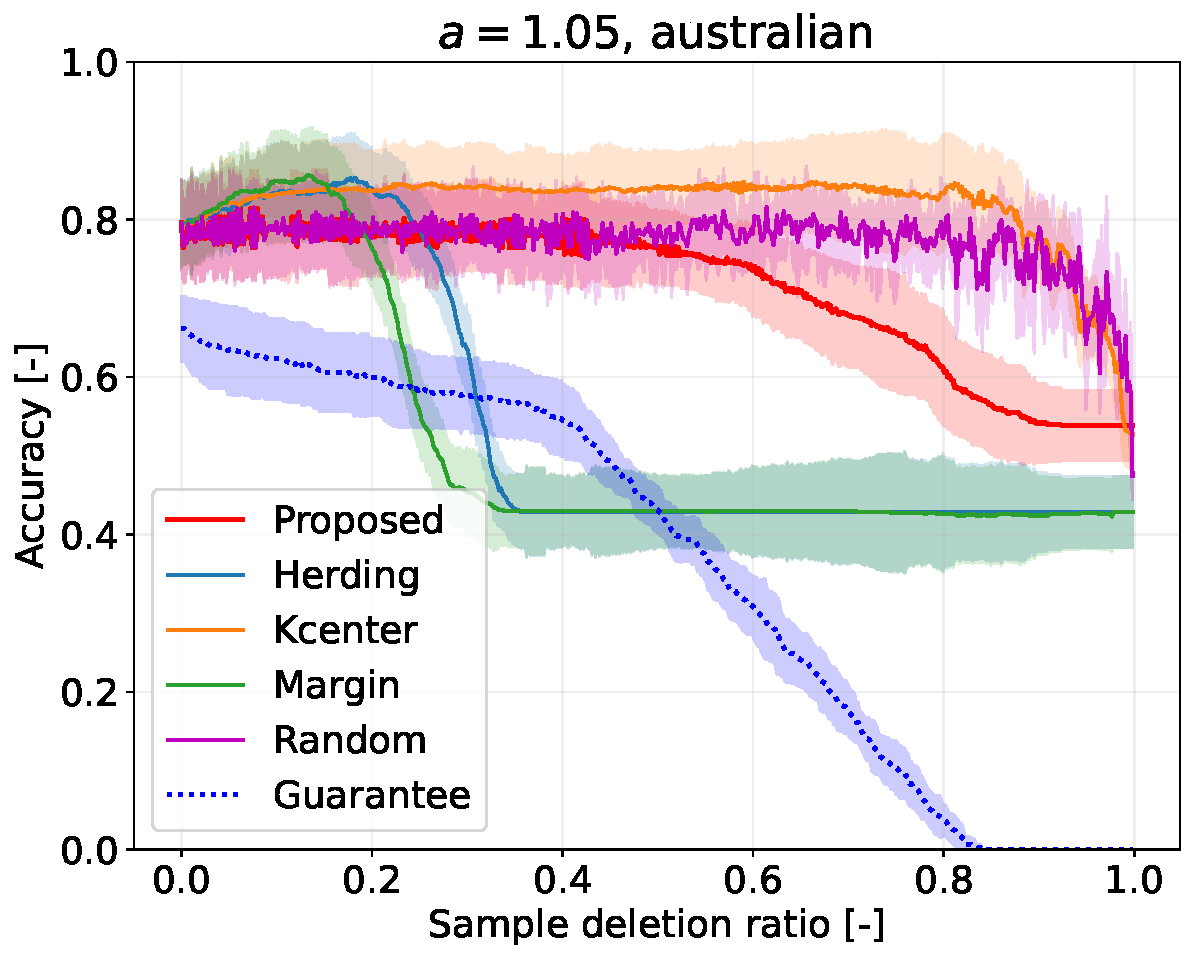
\includegraphics[width=0.8\hsize]{fig/table_logistic/australian-logistic/kernel/lam_552/a1.05000.pdf}\end{minipage}
		\\
		\begin{minipage}[b]{0.3\hsize}\centering {\small Dataset: breast-cancer, $\lambda=\lambda_\mathrm{best}$}\\\includegraphics[width=0.8\hsize]{fig/table_logistic/breast-cancer-logistic/kernel/lam_0.9/a1.05000.pdf}\end{minipage}
		&
		\begin{minipage}[b]{0.3\hsize}\centering {\small Dataset: breast-cancer, $\lambda=n \cdot 10^{-1.5}$}\\\includegraphics[width=0.8\hsize]{fig/table_logistic/breast-cancer-logistic/kernel/lam_17.26/a1.05000.pdf}\end{minipage}
		&
		\begin{minipage}[b]{0.3\hsize}\centering {\small Dataset: breast-cancer, $\lambda=n$}\\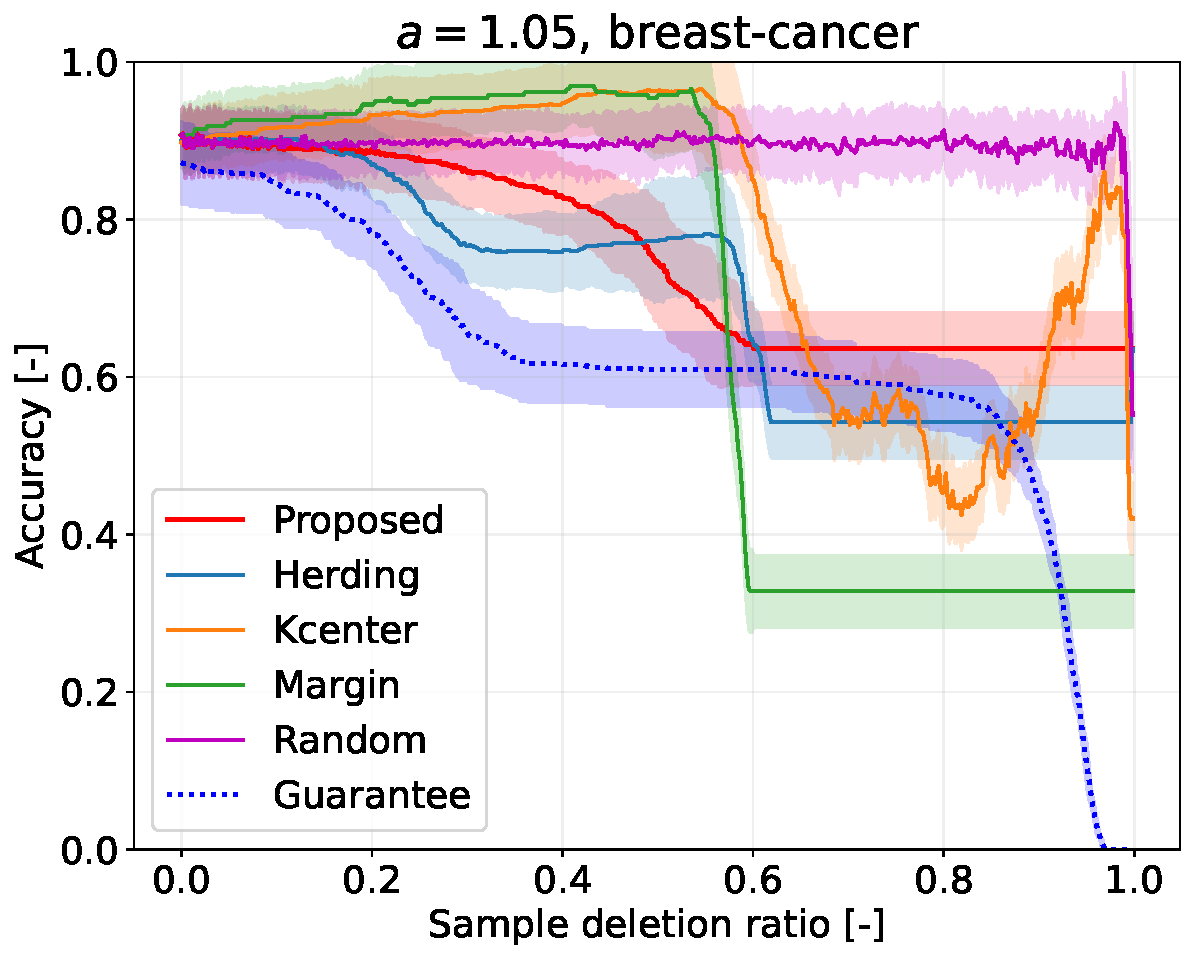
\includegraphics[width=0.8\hsize]{fig/table_logistic/breast-cancer-logistic/kernel/lam_546/a1.05000.pdf}\end{minipage}
		\\
		\begin{minipage}[b]{0.3\hsize}\centering {\small Dataset: heart, $\lambda=\lambda_\mathrm{best}$}\\\includegraphics[width=0.8\hsize]{fig/table_logistic/heart-logistic/kernel/lam_2.7/a1.05000.pdf}\end{minipage}
		&
		\begin{minipage}[b]{0.3\hsize}\centering {\small Dataset: heart, $\lambda=n \cdot 10^{-1.5}$}\\\includegraphics[width=0.8\hsize]{fig/table_logistic/heart-logistic/kernel/lam_6.830/a1.05000.pdf}\end{minipage}
		&
		\begin{minipage}[b]{0.3\hsize}\centering {\small Dataset: heart, $\lambda=n$}\\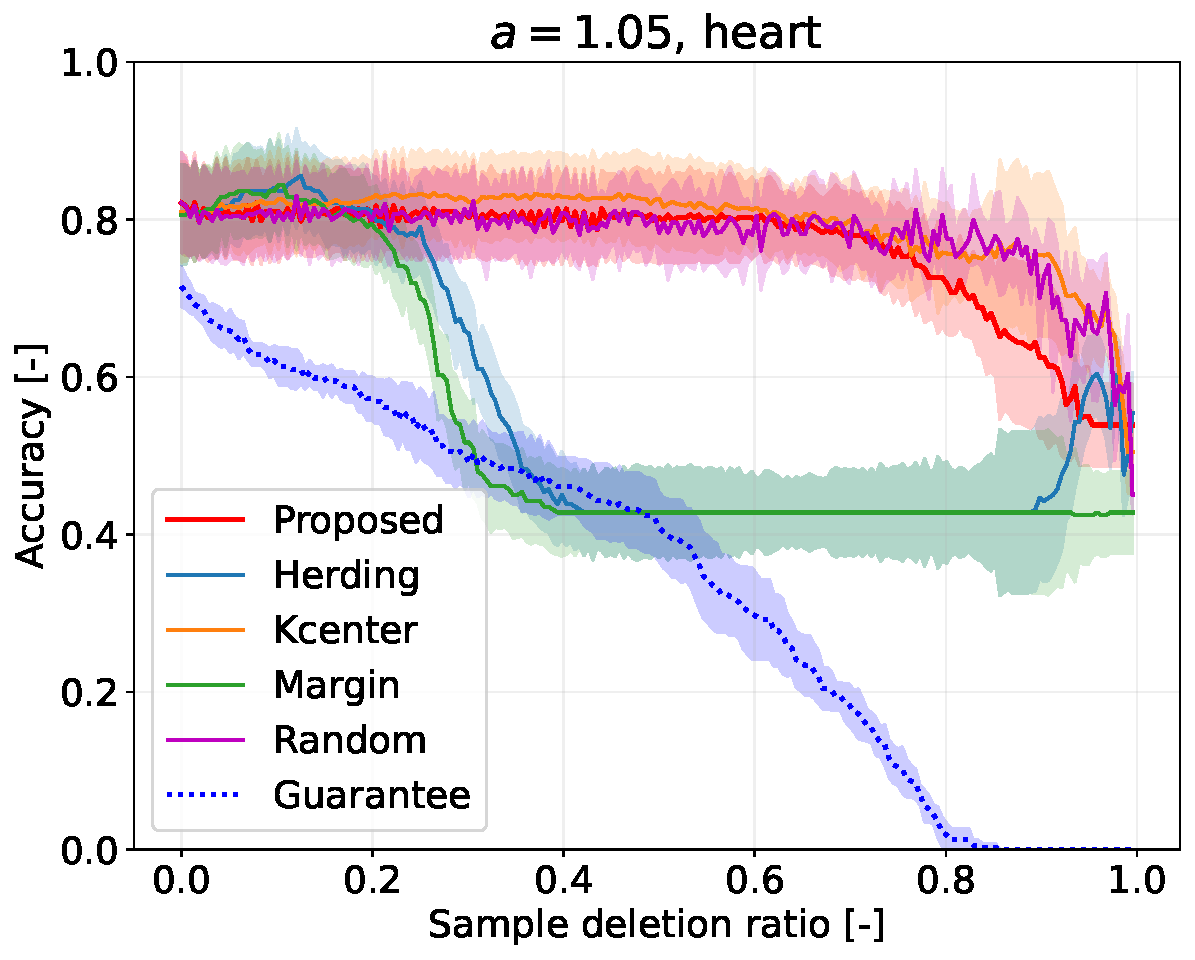
\includegraphics[width=0.8\hsize]{fig/table_logistic/heart-logistic/kernel/lam_216/a1.05000.pdf}\end{minipage}
		\\
		\begin{minipage}[b]{0.3\hsize}\centering {\small Dataset: ionosphere, $\lambda=\lambda_\mathrm{best}$}\\\includegraphics[width=0.8\hsize]{fig/table_logistic/ionosphere_scale-logistic/kernel/lam_0.28/a1.05000.pdf}\end{minipage}
		&
		\begin{minipage}[b]{0.3\hsize}\centering {\small Dataset: ionosphere, $\lambda=n \cdot 10^{-1.5}$}\\\includegraphics[width=0.8\hsize]{fig/table_logistic/ionosphere_scale-logistic/kernel/lam_8.854/a1.05000.pdf}\end{minipage}
		&
		\begin{minipage}[b]{0.3\hsize}\centering {\small Dataset: ionosphere, $\lambda=n$}\\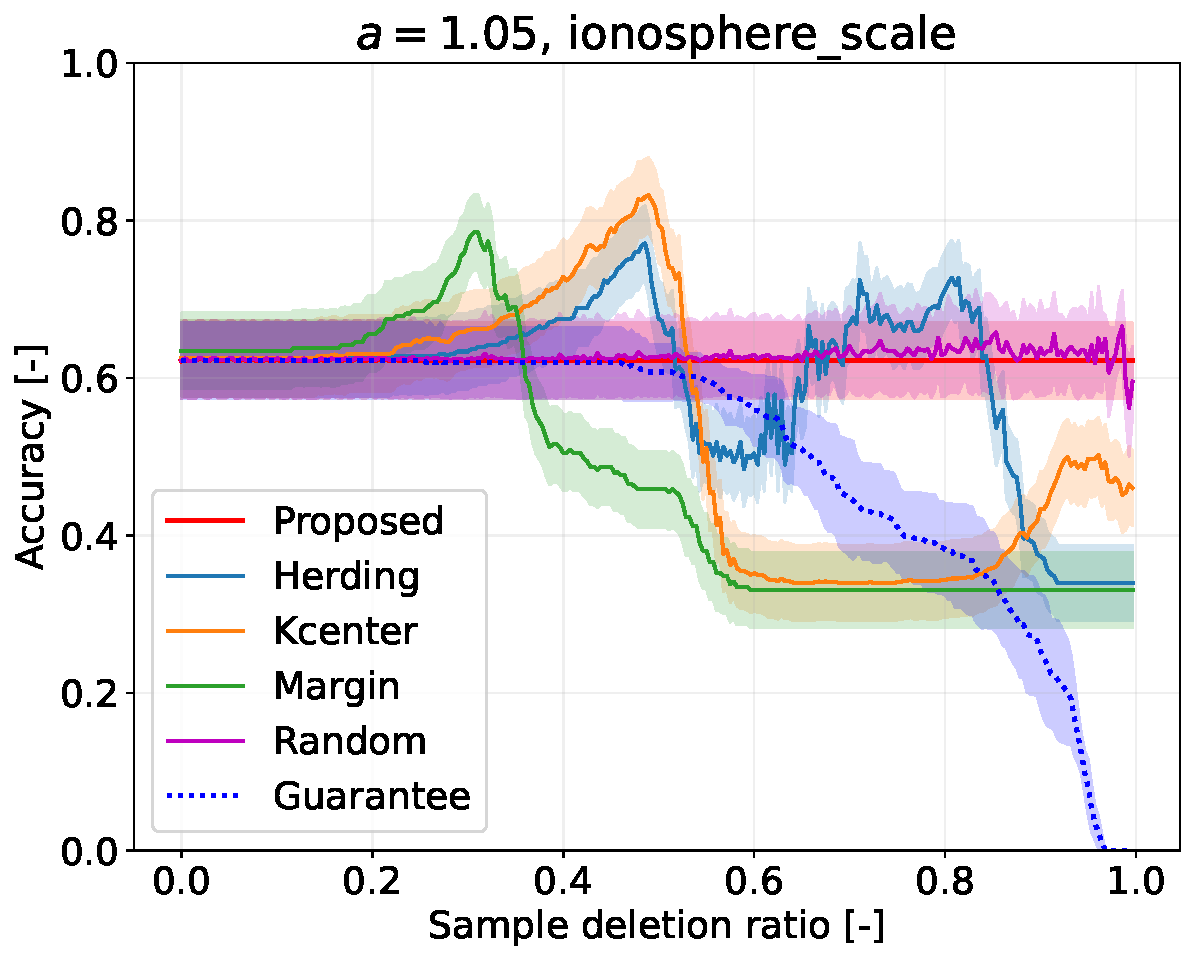
\includegraphics[width=0.8\hsize]{fig/table_logistic/ionosphere_scale-logistic/kernel/lam_280/a1.05000.pdf}\end{minipage}
		\\
		\begin{minipage}[b]{0.3\hsize}\centering {\small Dataset: splice, $\lambda=\lambda_\mathrm{best}$}\\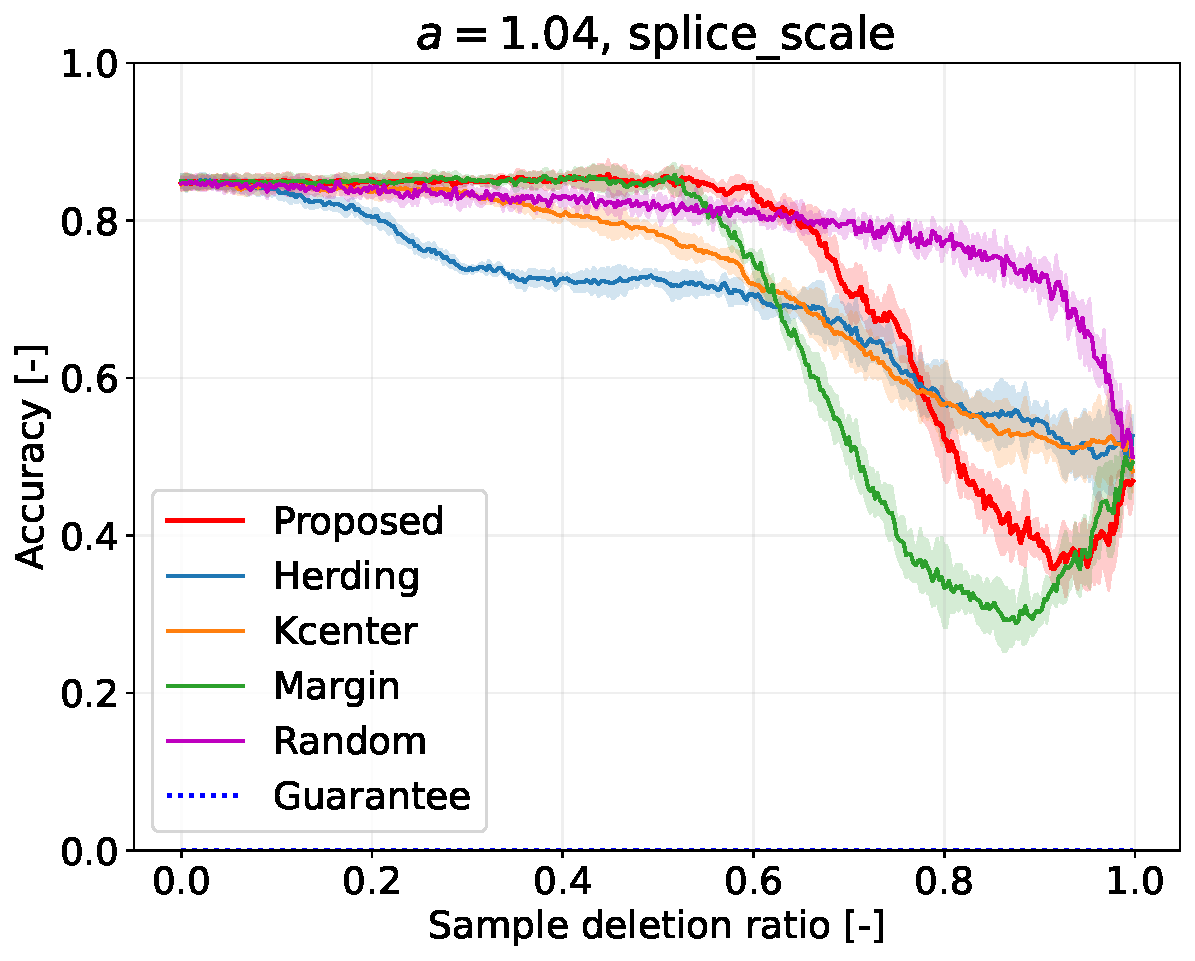
\includegraphics[width=0.8\hsize]{fig/table_logistic/splice_scale-logistic/kernel/lam_0.03/a1.04000.pdf}\end{minipage}
		&
		\begin{minipage}[b]{0.3\hsize}\centering {\small Dataset: splice, $\lambda=n_\mathrm \cdot 10^{-1.5}$}\\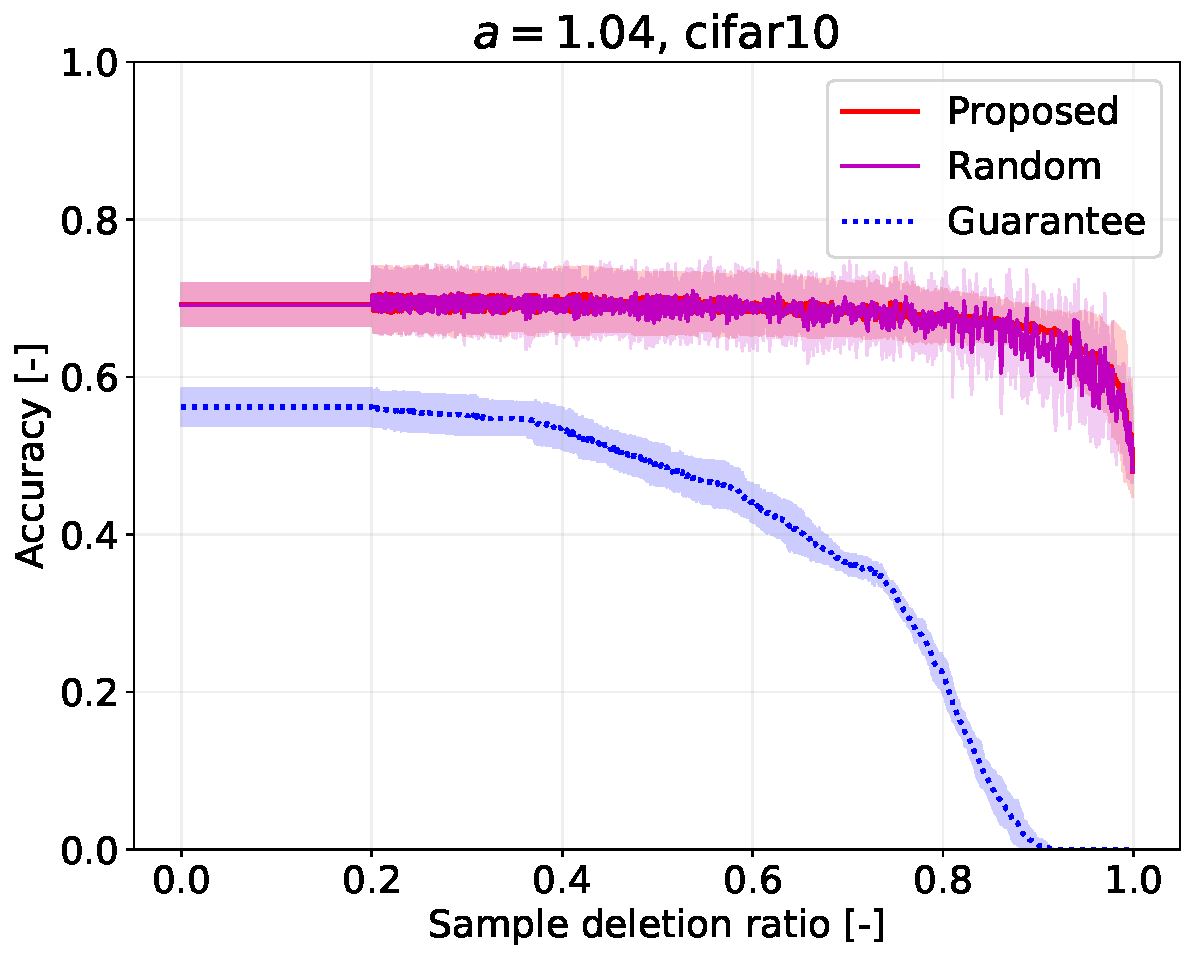
\includegraphics[width=0.8\hsize]{fig/table_logistic/splice_scale-logistic/kernel/lam_25.29/a1.04000.pdf}\end{minipage}
		&
		\begin{minipage}[b]{0.3\hsize}\centering {\small Dataset: splice, $\lambda=n$}\\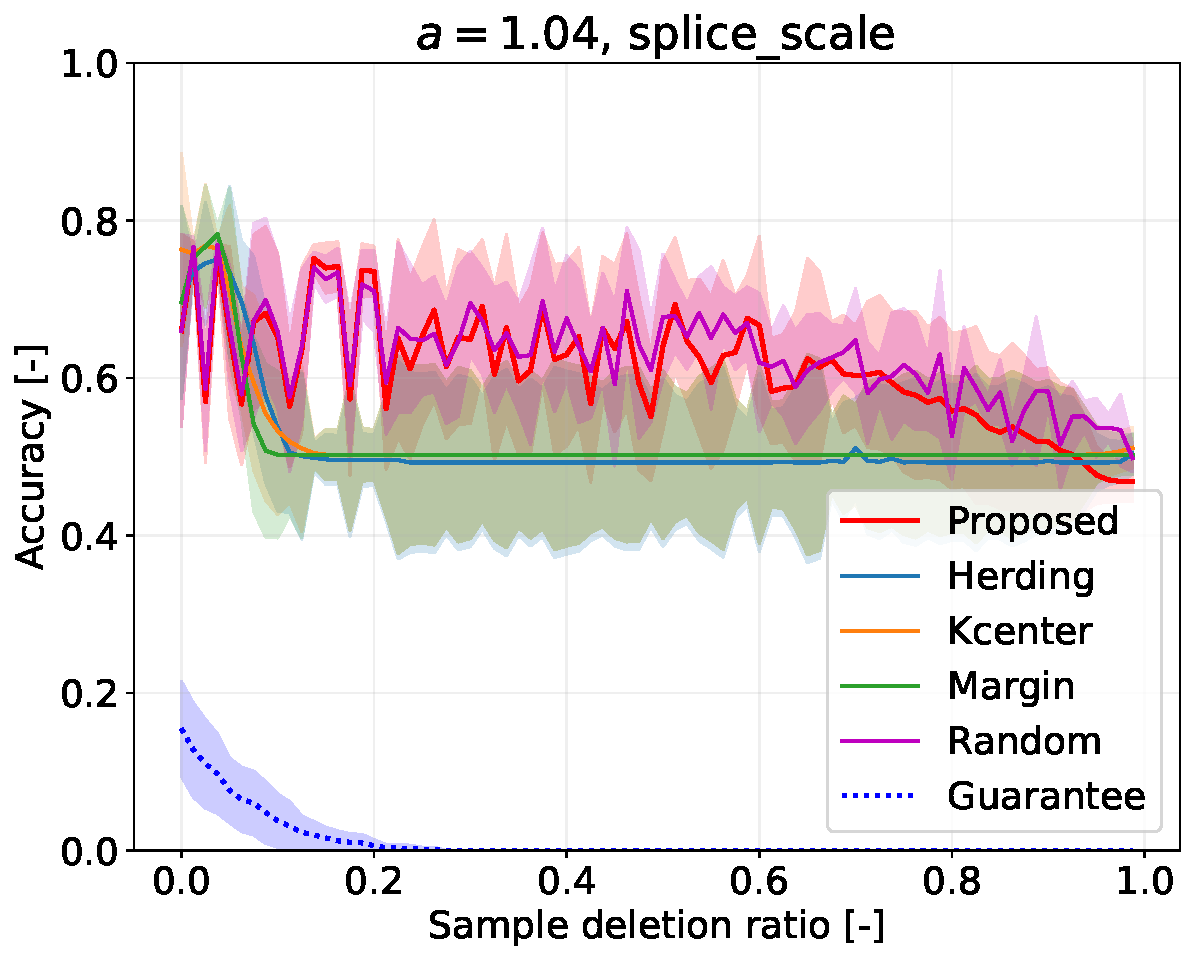
\includegraphics[width=0.8\hsize]{fig/table_logistic/splice_scale-logistic/kernel/lam_800/a1.04000.pdf}\end{minipage}
		\\
	
	\end{tabular}
	\caption{Model performance for RBF-kernel logistic regression models, under the settings described in Section \ref{sec:experiment} and Appendix \ref{app:experimental-setup}.}
	\label{fig:result-acc-logistic}
	\end{figure}


Next, we show a guarantee of model performance.


\begin{figure}[H]
	\begin{tabular}{ccc}
		\begin{minipage}[b]{0.3\hsize}\centering {\small Dataset: australian, $\lambda=n \cdot 10^{-3}$}\\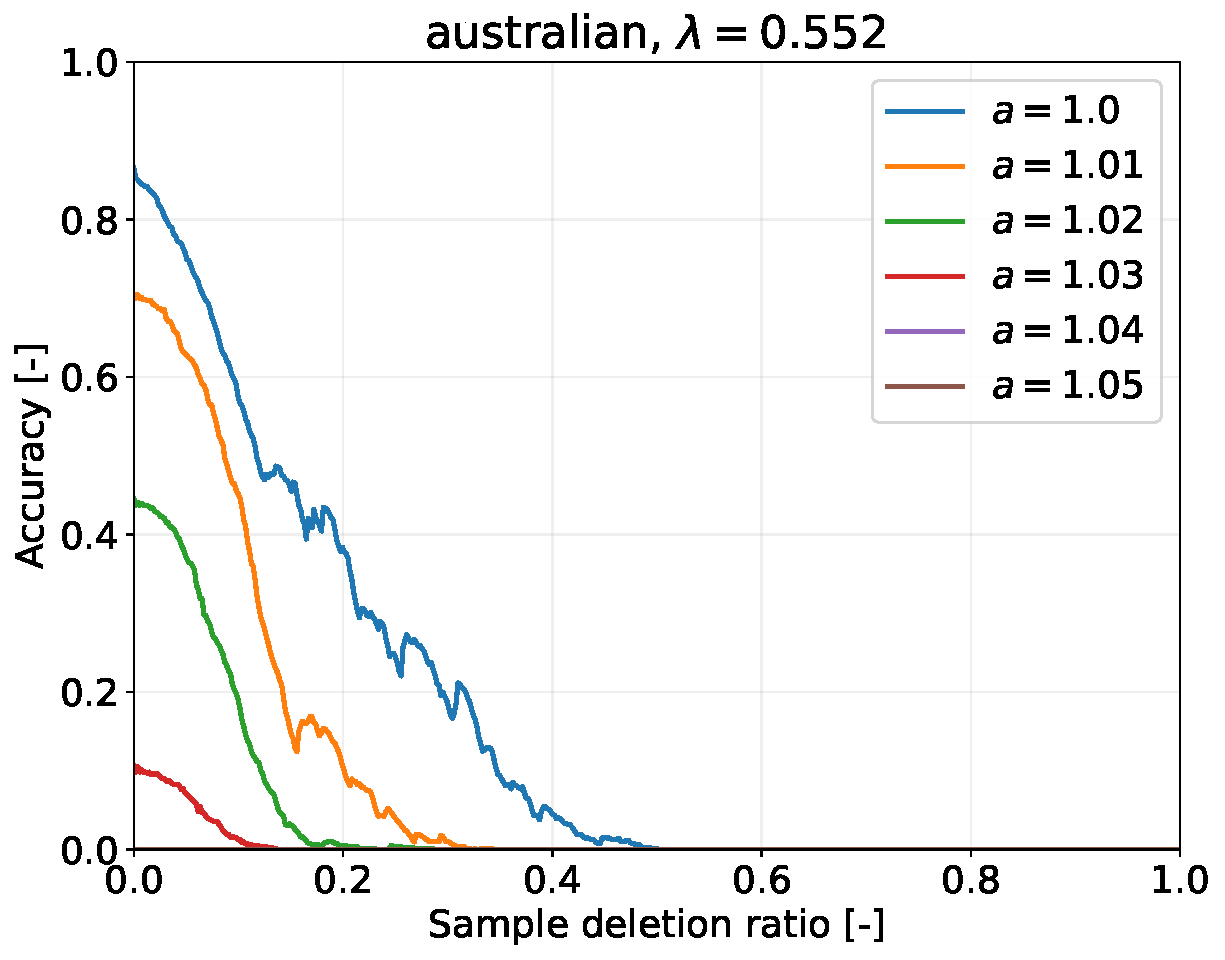
\includegraphics[width=0.8\hsize]{fig/table_logistic/australian-logistic/kernel/kernel_ss_screening_rate_lam0.552_x_n_y_etest.pdf}\end{minipage}
		&
		\begin{minipage}[b]{0.3\hsize}\centering {\small Dataset: australian, $\lambda=n \cdot 10^{-1.5}$}\\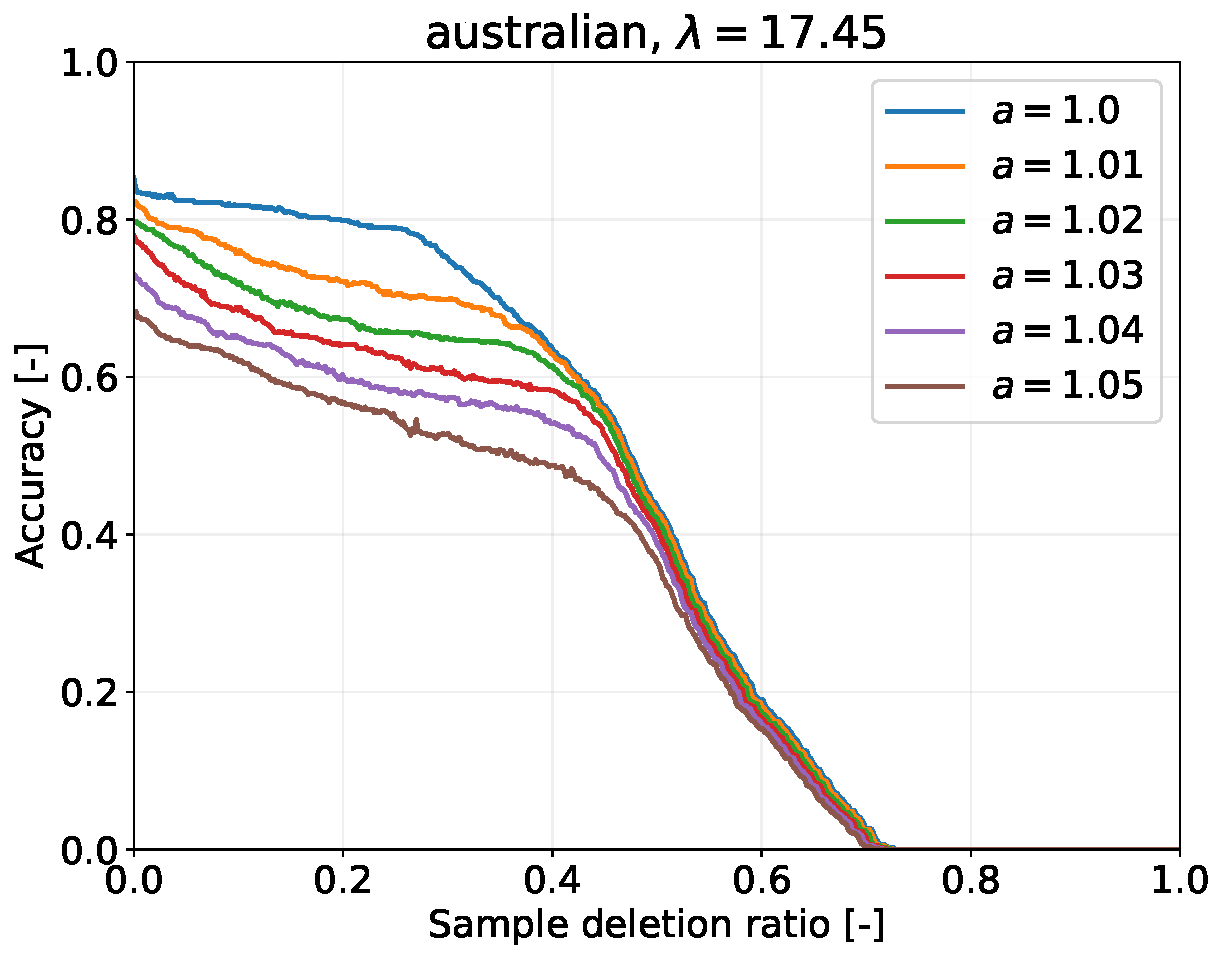
\includegraphics[width=0.8\hsize]{fig/table_logistic/australian-logistic/kernel/kernel_ss_screening_rate_lam17.45_x_n_y_etest.pdf}\end{minipage}
		&
		\begin{minipage}[b]{0.3\hsize}\centering {\small Dataset: australian, $\lambda=n$}\\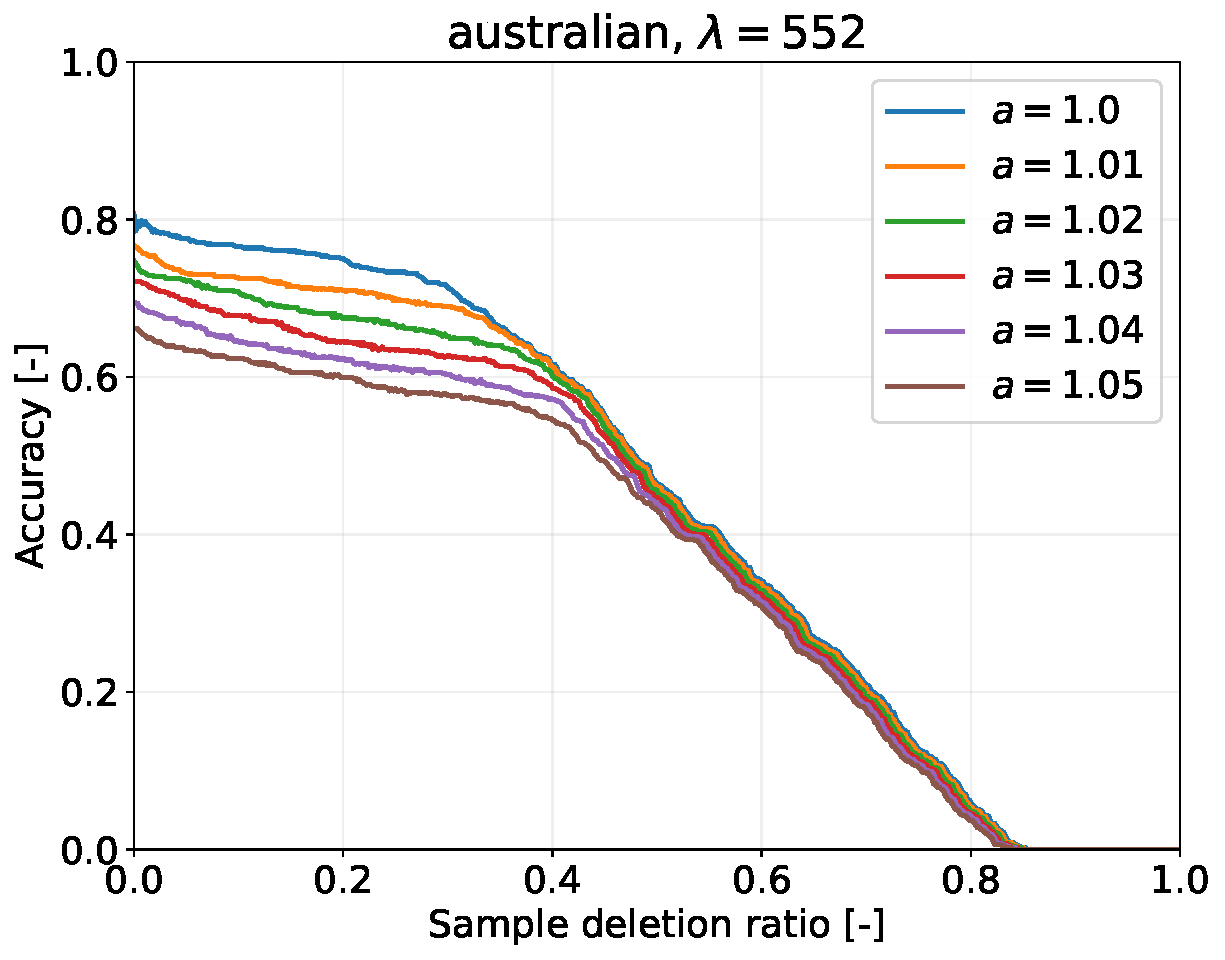
\includegraphics[width=0.8\hsize]{fig/table_logistic/australian-logistic/kernel/kernel_ss_screening_rate_lam552_x_n_y_etest.pdf}\end{minipage}
		\\
		\begin{minipage}[b]{0.3\hsize}\centering {\small Dataset: breast-cancer, $\lambda=n \cdot 10^{-3}$}\\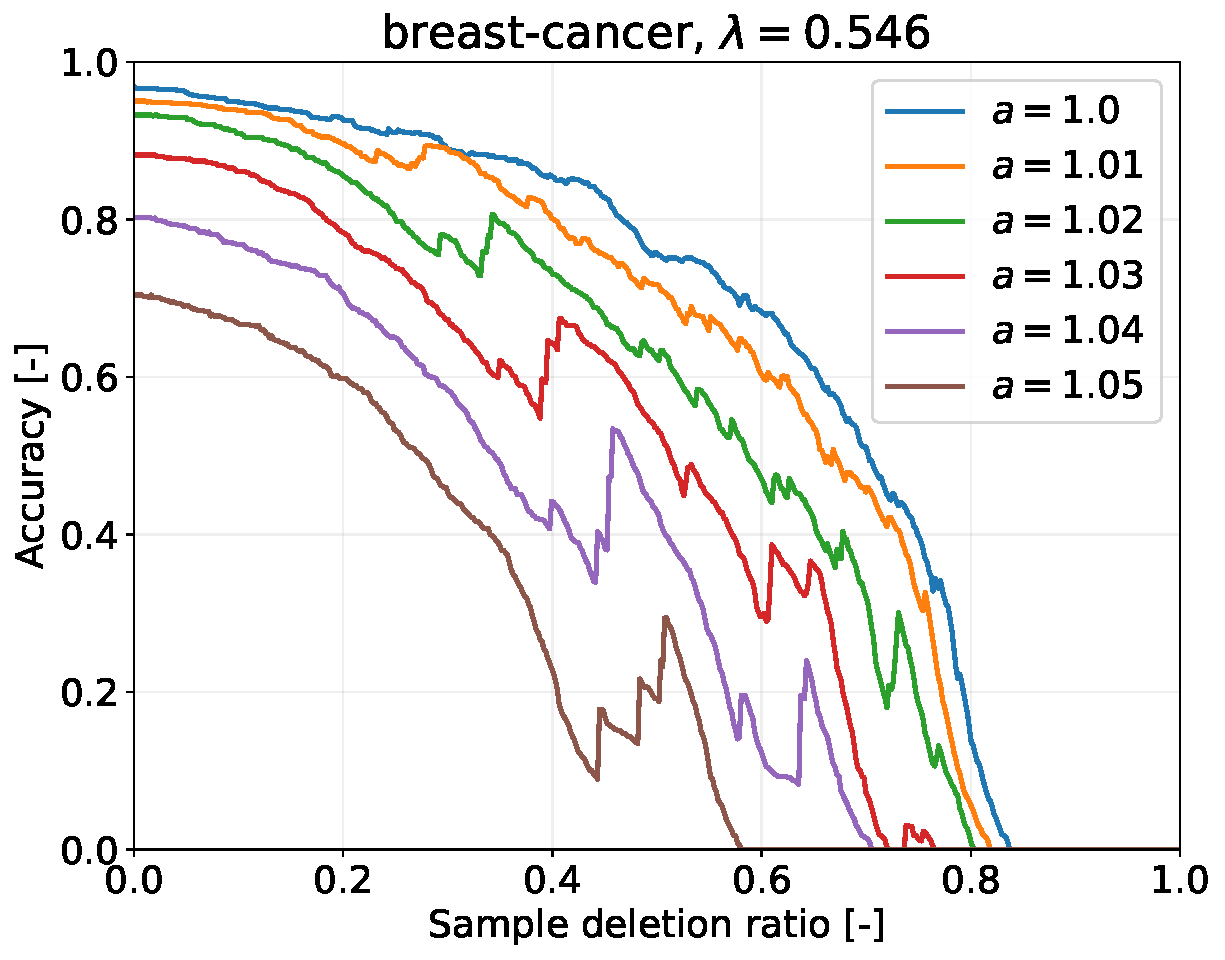
\includegraphics[width=0.8\hsize]{fig/table_logistic/breast-cancer-logistic/kernel/kernel_ss_screening_rate_lam0.546_x_n_y_etest.pdf}\end{minipage}
		&
		\begin{minipage}[b]{0.3\hsize}\centering {\small Dataset: breast-cancer, $\lambda=n \cdot 10^{-1.5}$}\\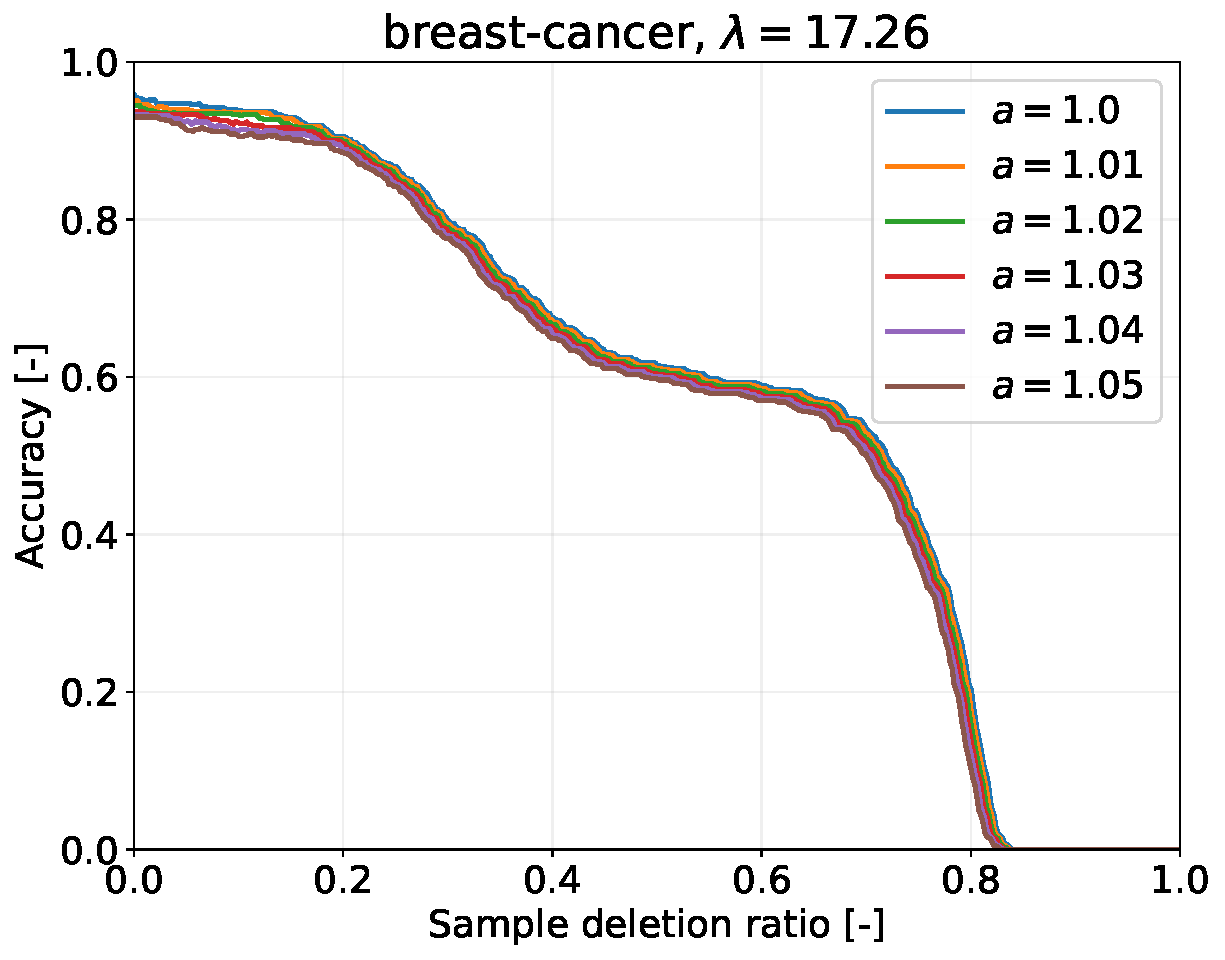
\includegraphics[width=0.8\hsize]{fig/table_logistic/breast-cancer-logistic/kernel/kernel_ss_screening_rate_lam17.26_x_n_y_etest.pdf}\end{minipage}
		&
		\begin{minipage}[b]{0.3\hsize}\centering {\small Dataset: breast-cancer, $\lambda=n$}\\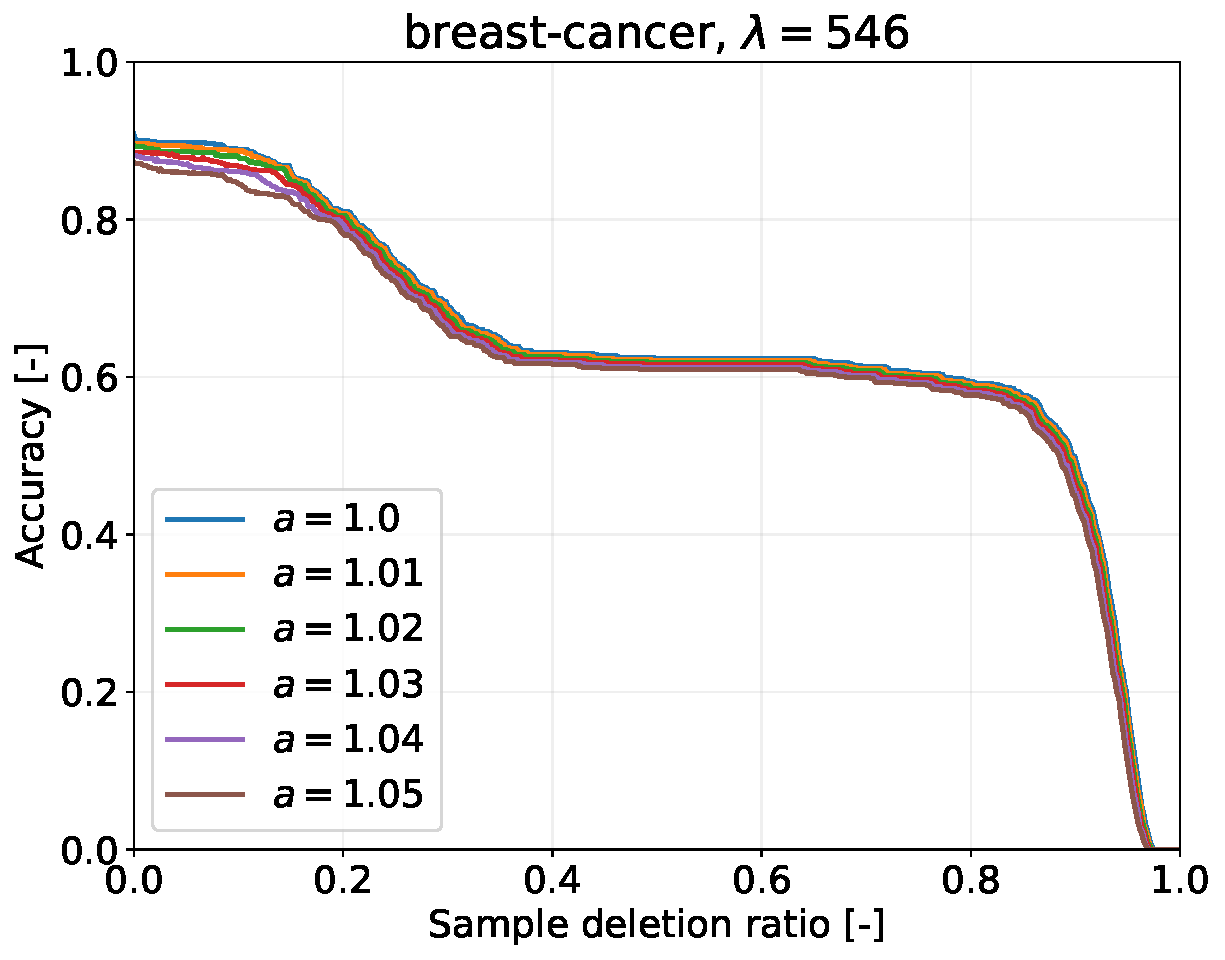
\includegraphics[width=0.8\hsize]{fig/table_logistic/breast-cancer-logistic/kernel/kernel_ss_screening_rate_lam546_x_n_y_etest.pdf}\end{minipage}
		\\
		\begin{minipage}[b]{0.3\hsize}\centering {\small Dataset: heart, $\lambda=n \cdot 10^{-3}$}\\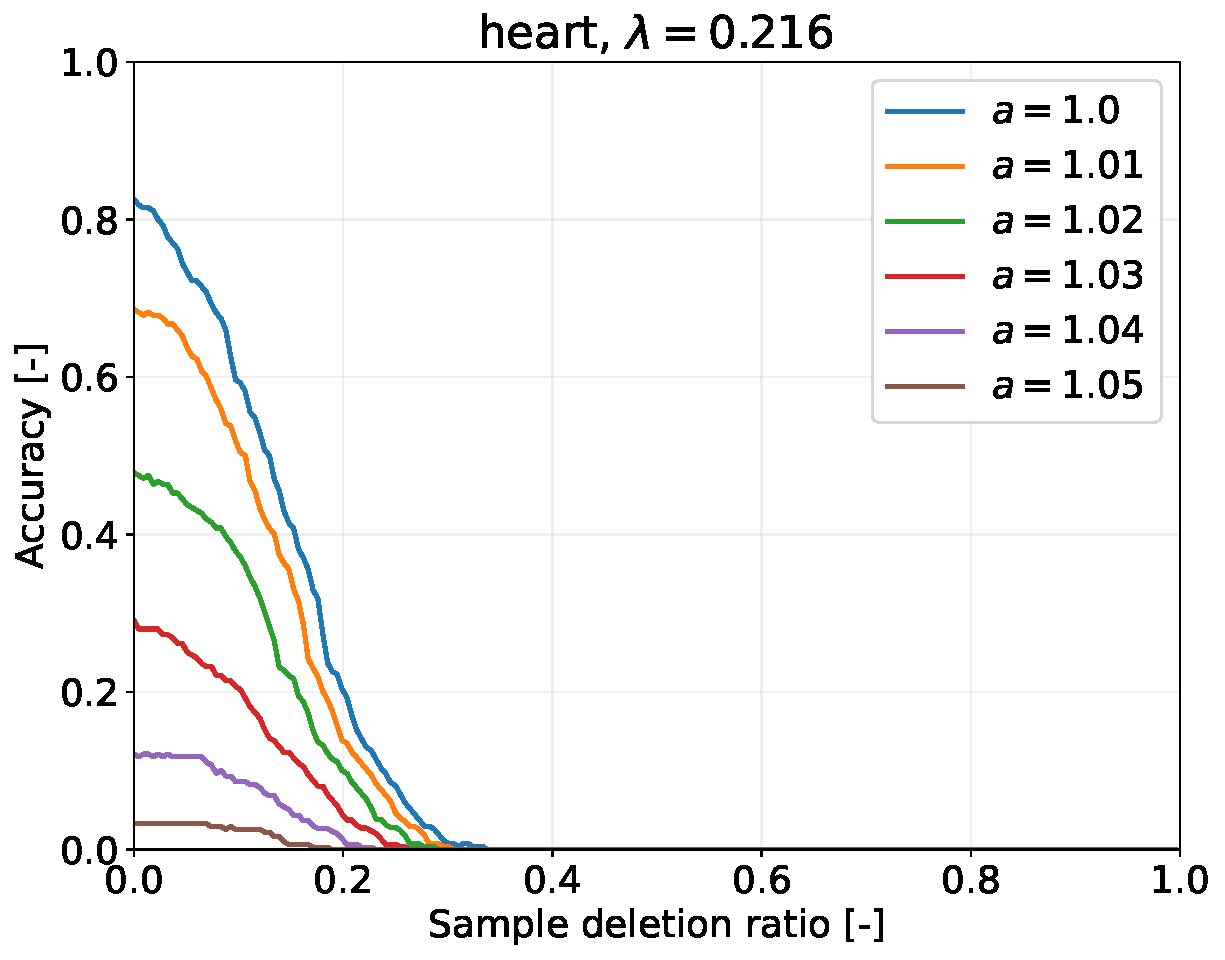
\includegraphics[width=0.8\hsize]{fig/table_logistic/heart-logistic/kernel/kernel_ss_screening_rate_lam0.216_x_n_y_etest.pdf}\end{minipage}
		&
		\begin{minipage}[b]{0.3\hsize}\centering {\small Dataset: heart, $\lambda=n \cdot 10^{-1.5}$}\\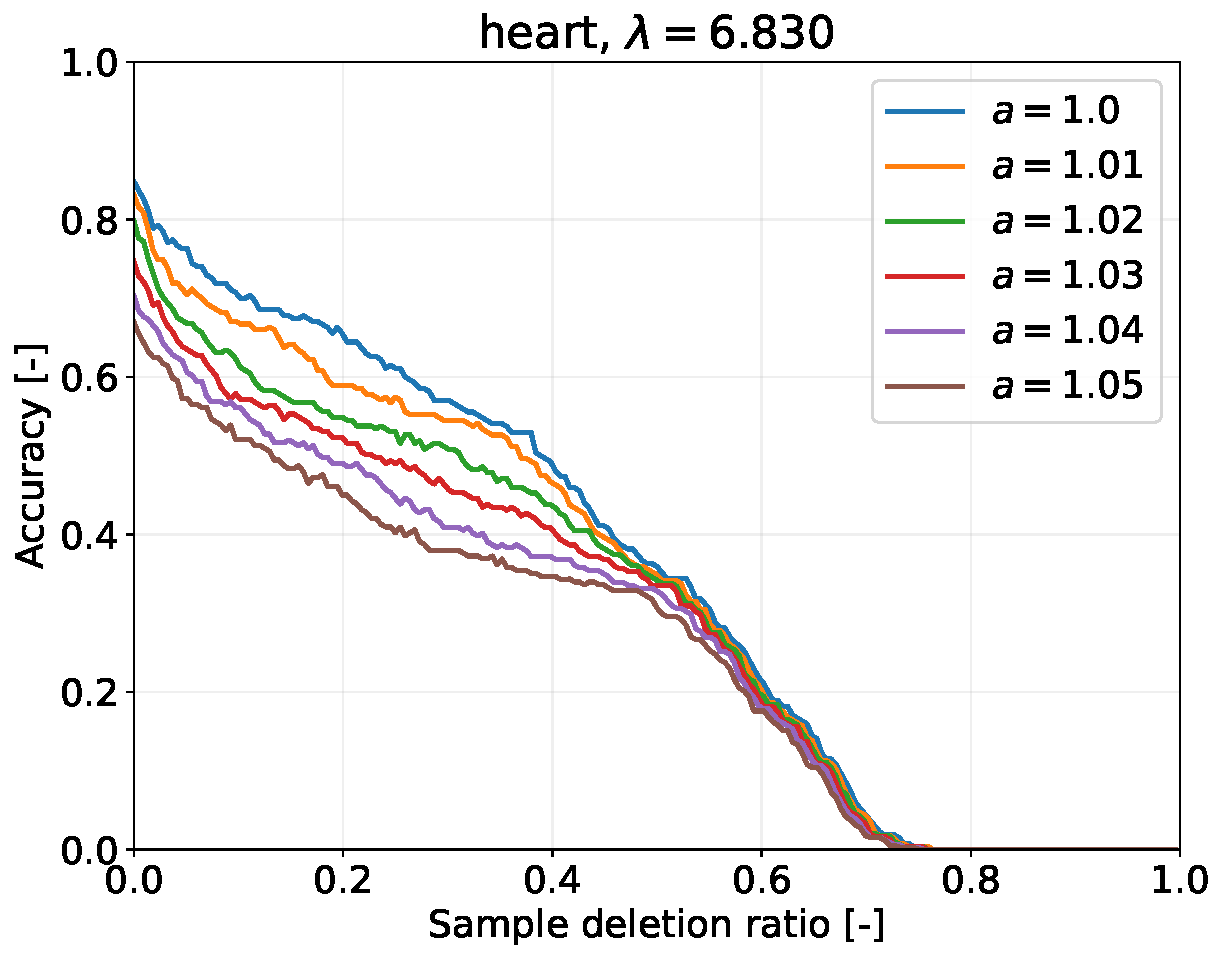
\includegraphics[width=0.8\hsize]{fig/table_logistic/heart-logistic/kernel/kernel_ss_screening_rate_lam6.830_x_n_y_etest.pdf}\end{minipage}
		&
		\begin{minipage}[b]{0.3\hsize}\centering {\small Dataset: heart, $\lambda=n$}\\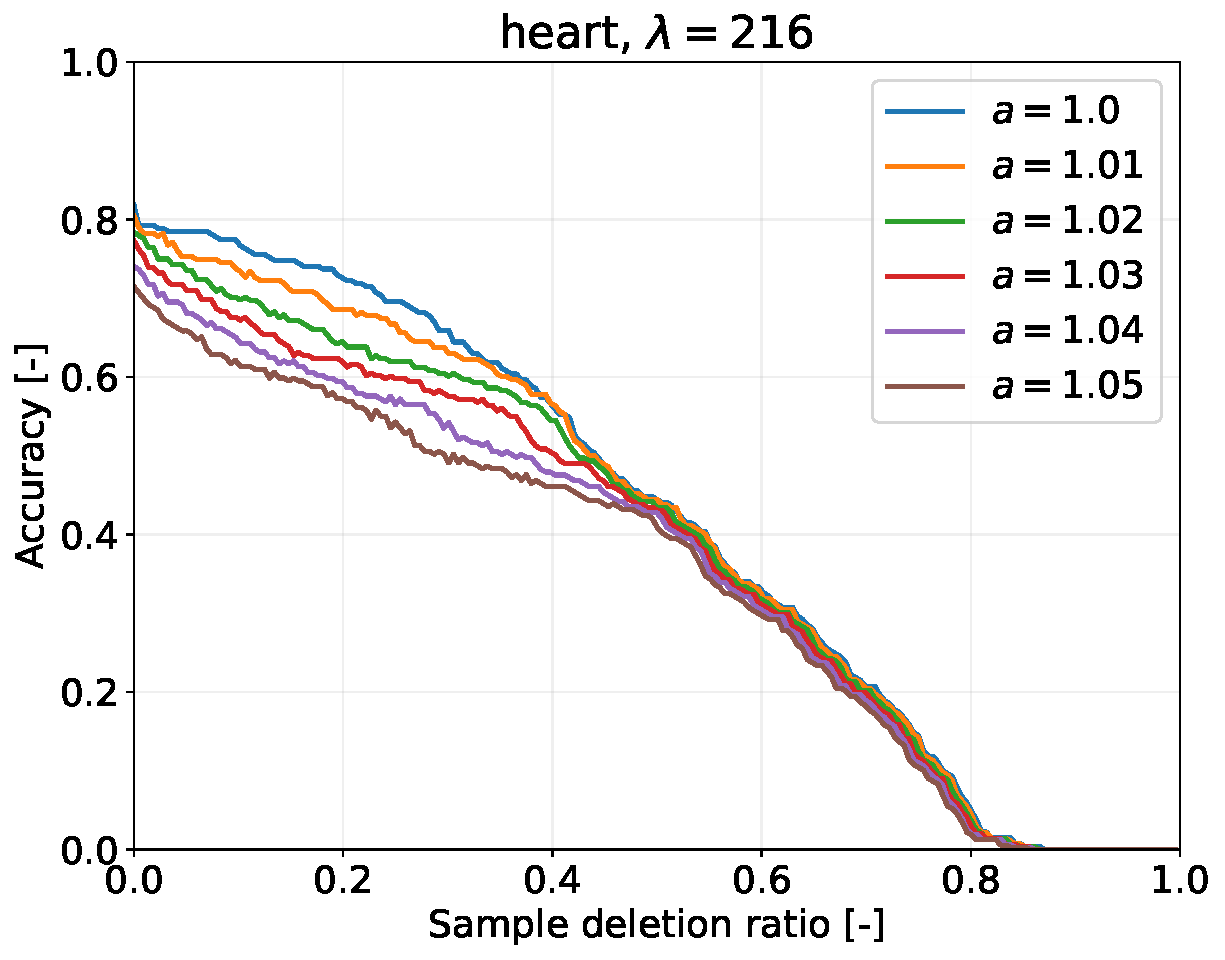
\includegraphics[width=0.8\hsize]{fig/table_logistic/heart-logistic/kernel/kernel_ss_screening_rate_lam216_x_n_y_etest.pdf}\end{minipage}
		\\
		\begin{minipage}[b]{0.3\hsize}\centering {\small Dataset: ionosphere, $\lambda=n \cdot 10^{-3}$}\\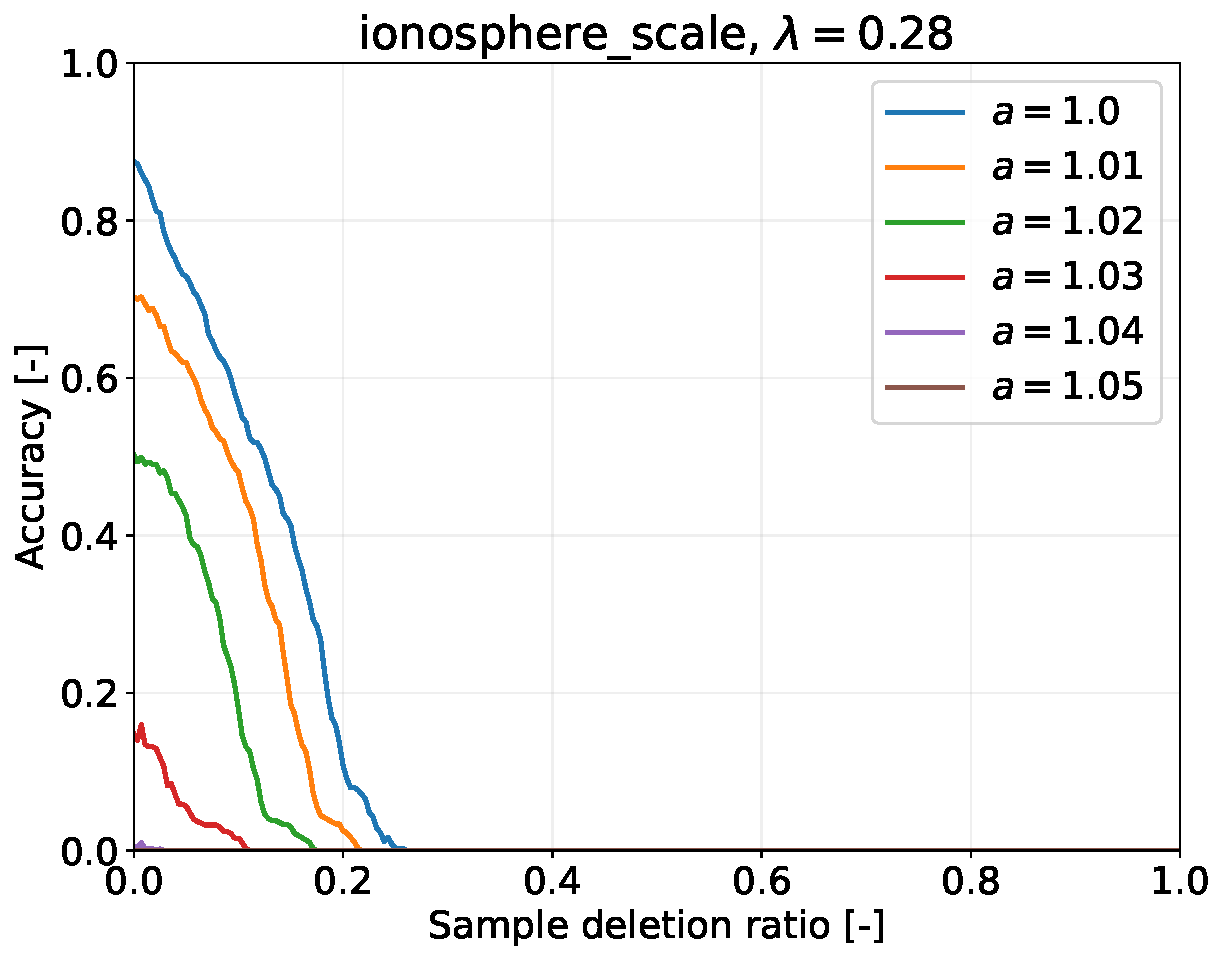
\includegraphics[width=0.8\hsize]{fig/table_logistic/ionosphere_scale-logistic/kernel/kernel_ss_screening_rate_lam0.28_x_n_y_etest.pdf}\end{minipage}
		&
		\begin{minipage}[b]{0.3\hsize}\centering {\small Dataset: ionosphere, $\lambda=n \cdot 10^{-1.5}$}\\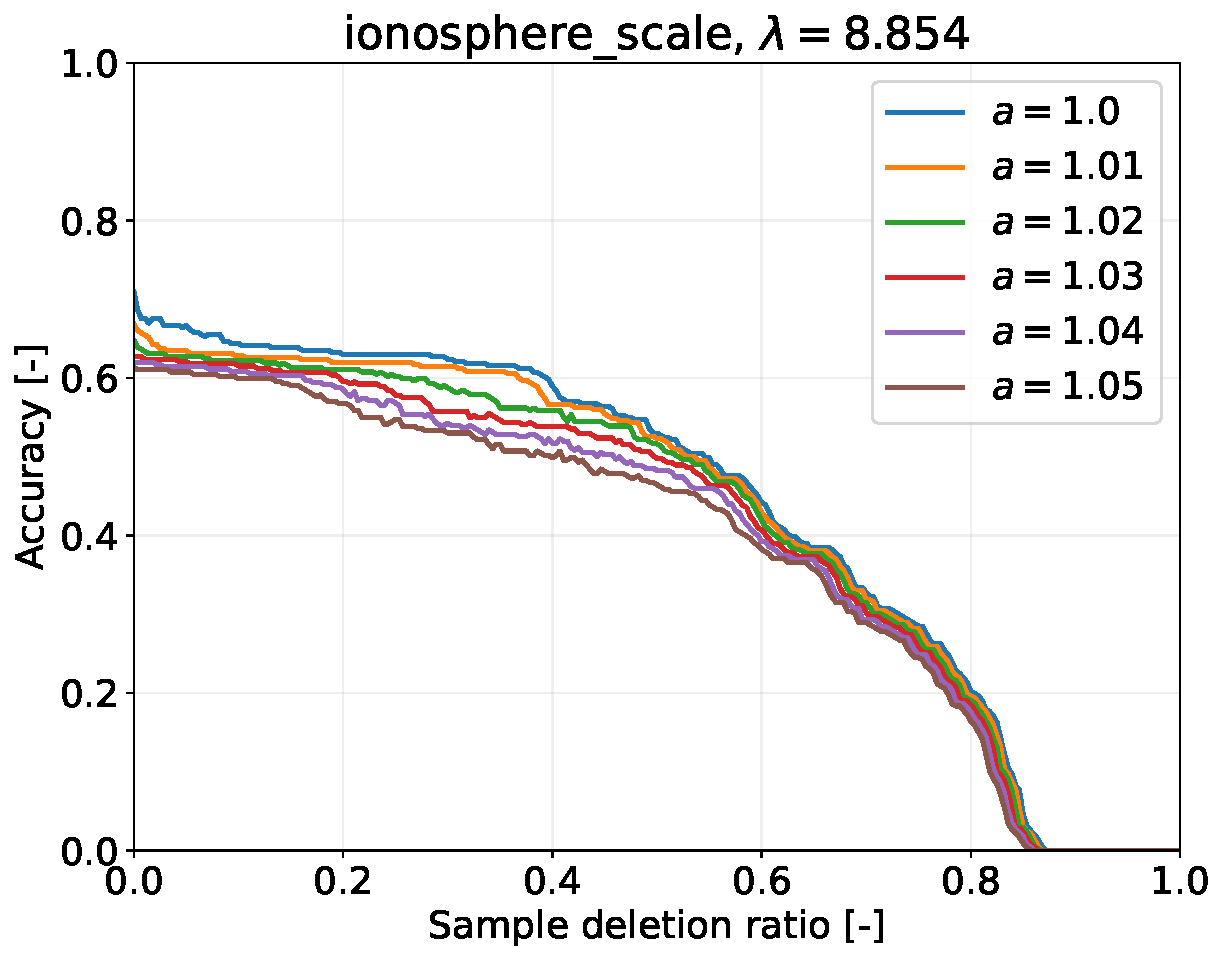
\includegraphics[width=0.8\hsize]{fig/table_logistic/ionosphere_scale-logistic/kernel/kernel_ss_screening_rate_lam8.854_x_n_y_etest.pdf}\end{minipage}
		&
		\begin{minipage}[b]{0.3\hsize}\centering {\small Dataset: ionosphere, $\lambda=n$}\\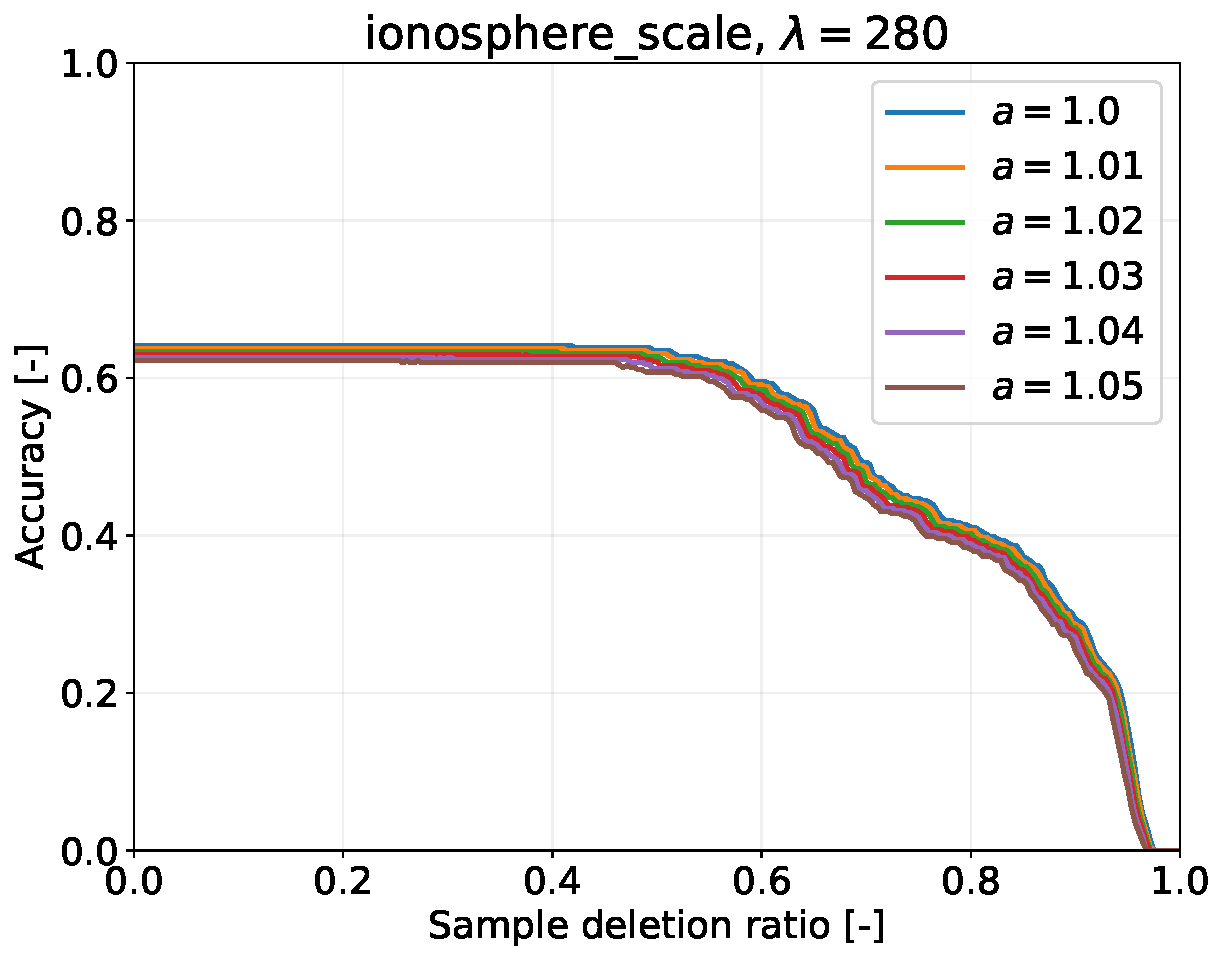
\includegraphics[width=0.8\hsize]{fig/table_logistic/ionosphere_scale-logistic/kernel/kernel_ss_screening_rate_lam280_x_n_y_etest.pdf}\end{minipage}
		\\
		\begin{minipage}[b]{0.3\hsize}\centering {\small Dataset: splice, $\lambda=n \cdot 10^{-3}$}\\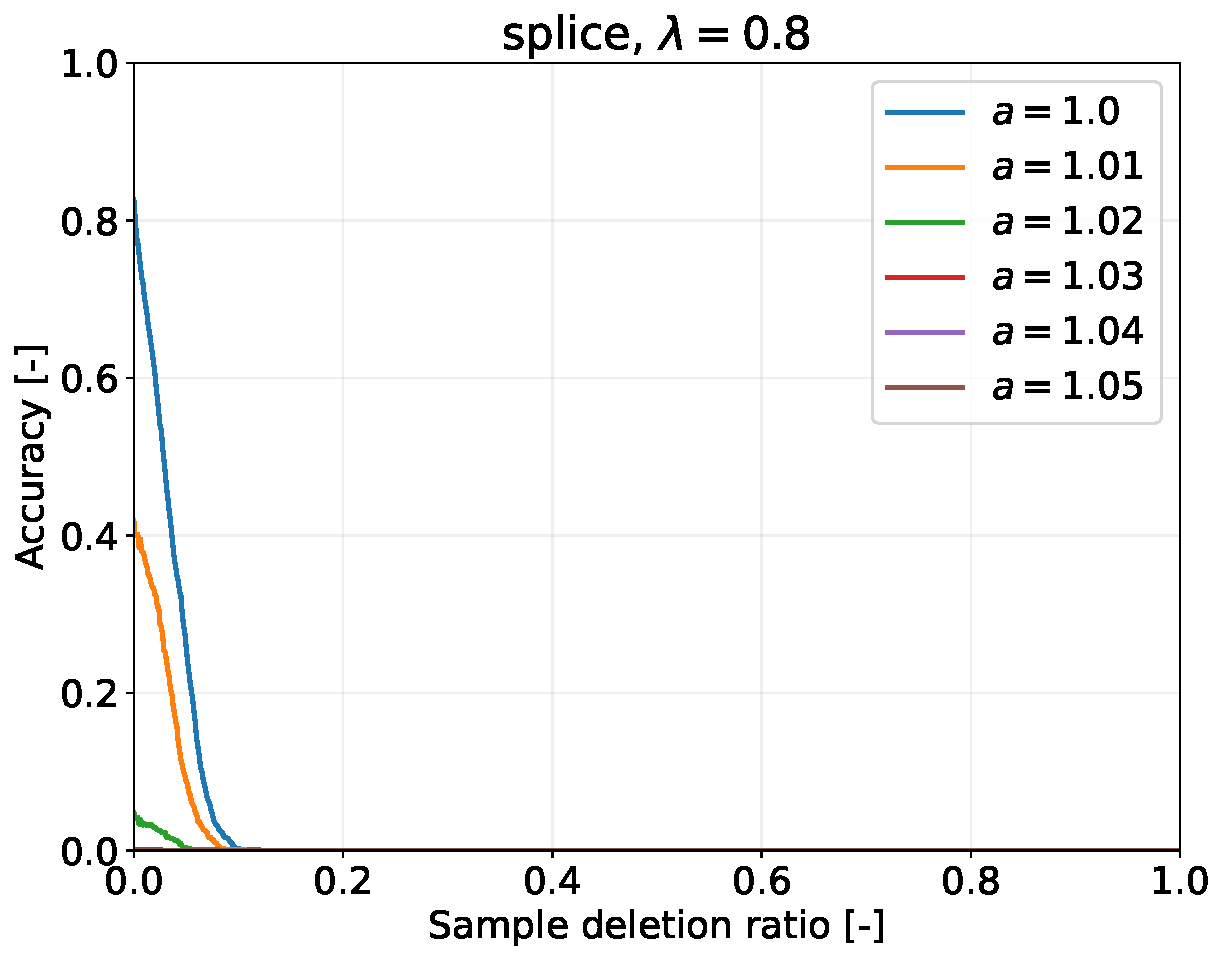
\includegraphics[width=0.8\hsize]{fig/table_logistic/splice_scale-logistic/kernel/kernel_ss_screening_rate_lam0.8_x_n_y_etest.pdf}\end{minipage}
		&
		\begin{minipage}[b]{0.3\hsize}\centering {\small Dataset: splice, $\lambda=n_\mathrm \cdot 10^{-1.5}$}\\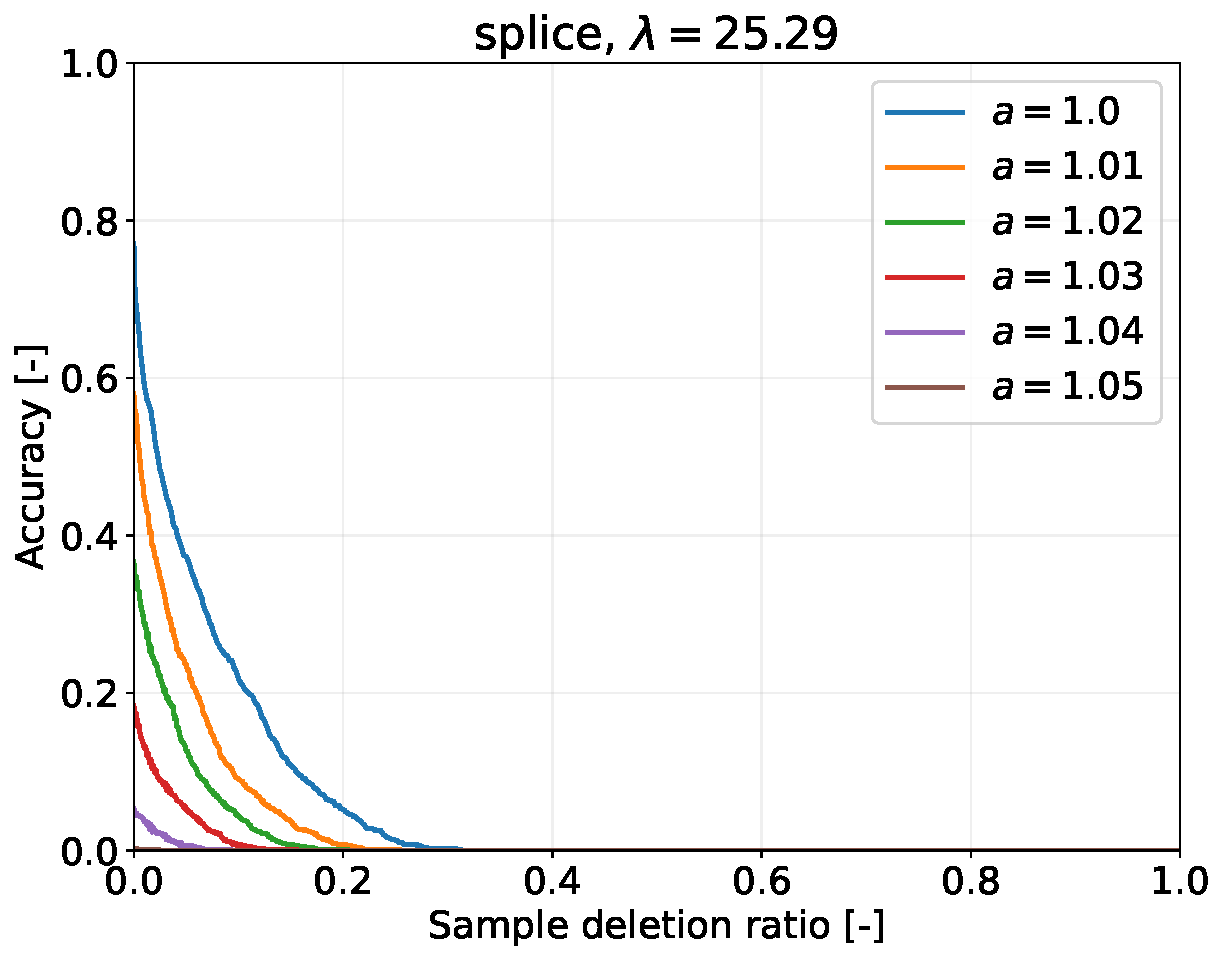
\includegraphics[width=0.8\hsize]{fig/table_logistic/splice_scale-logistic/kernel/kernel_ss_screening_rate_lam25.29_x_n_y_etest.pdf}\end{minipage}
		&
		\begin{minipage}[b]{0.3\hsize}\centering {\small Dataset: splice, $\lambda=n$}\\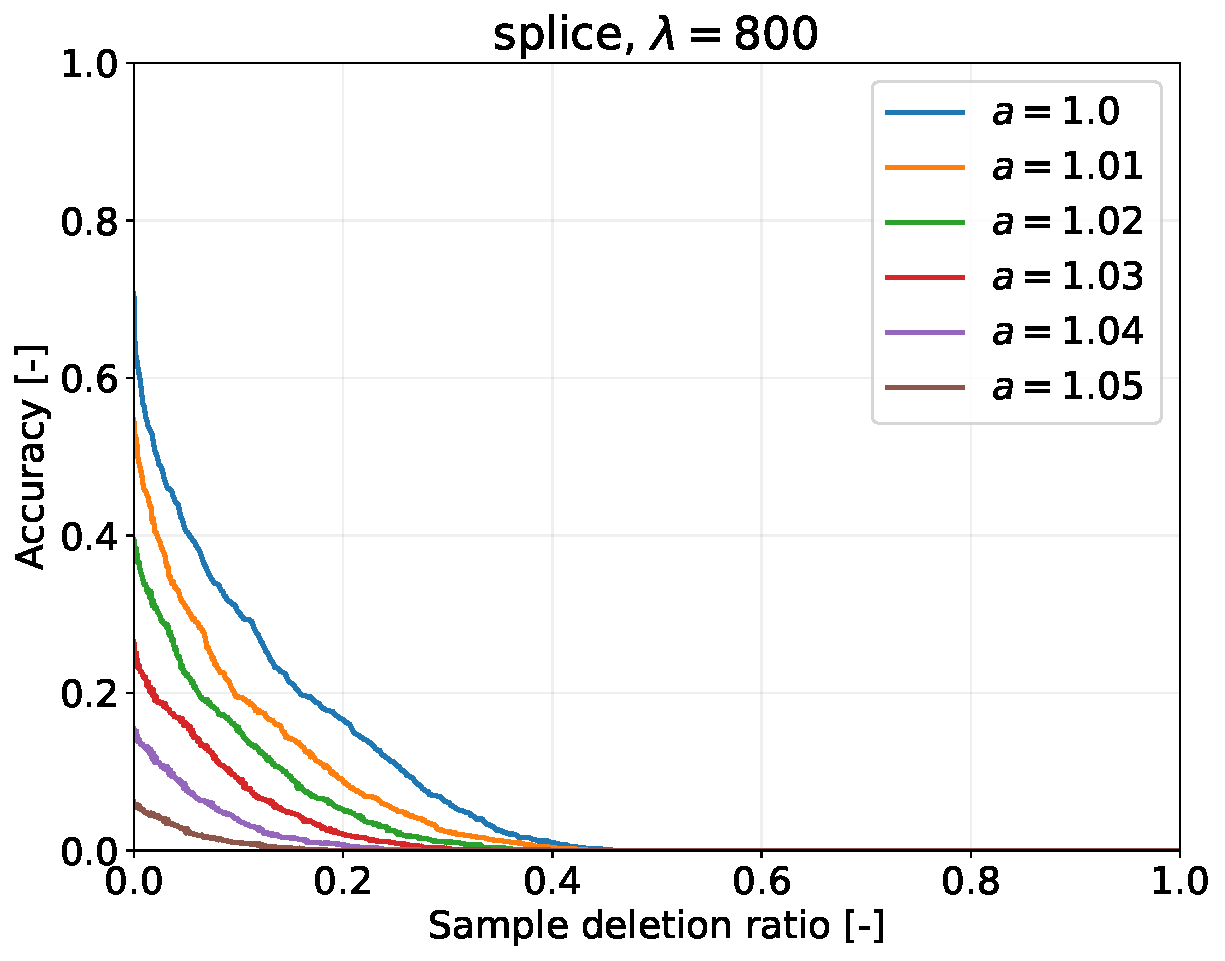
\includegraphics[width=0.8\hsize]{fig/table_logistic/splice_scale-logistic/kernel/kernel_ss_screening_rate_lam800_x_n_y_etest.pdf}\end{minipage}
		\\
	
	\end{tabular}
	\caption{Model performance for RBF-kernel logistic regression models, under the settings described in Section \ref{sec:experiment} and Appendix \ref{app:experimental-setup}.}
	\label{fig:result-guarantee-logistic}
	\end{figure}

	\newpage
% % % % % % % % % % % % % % % % % % % % % % % % % % % % % %
\subsection{All Experimental Results of Section \ref{subsec:result-table} using support vector machine model} \label{app:result-svm}
% % % % % % % % % % % % % % % % % % % % % % % % % % % % % %

In this appendix~\ref{app:result-svm}, we show all experimental results using support vector machine model(hinge loss + L2 reguralization). First, we show model performance.

\begin{figure}[H]
\begin{tabular}{ccc}
	\begin{minipage}[b]{0.3\hsize}\centering {\small Dataset: australian, $\lambda=\lambda_\mathrm{best}$}\\\includegraphics[width=0.8\hsize]{fig/australian/lam_11.0/a1.05000.pdf}\end{minipage}
	&
	\begin{minipage}[b]{0.3\hsize}\centering {\small Dataset: australian, $\lambda=n \cdot 10^{-1.5}$}\\\includegraphics[width=0.8\hsize]{fig/australian/lam_17.45/a1.05000.pdf}\end{minipage}
	&
	\begin{minipage}[b]{0.3\hsize}\centering {\small Dataset: australian, $\lambda=n$}\\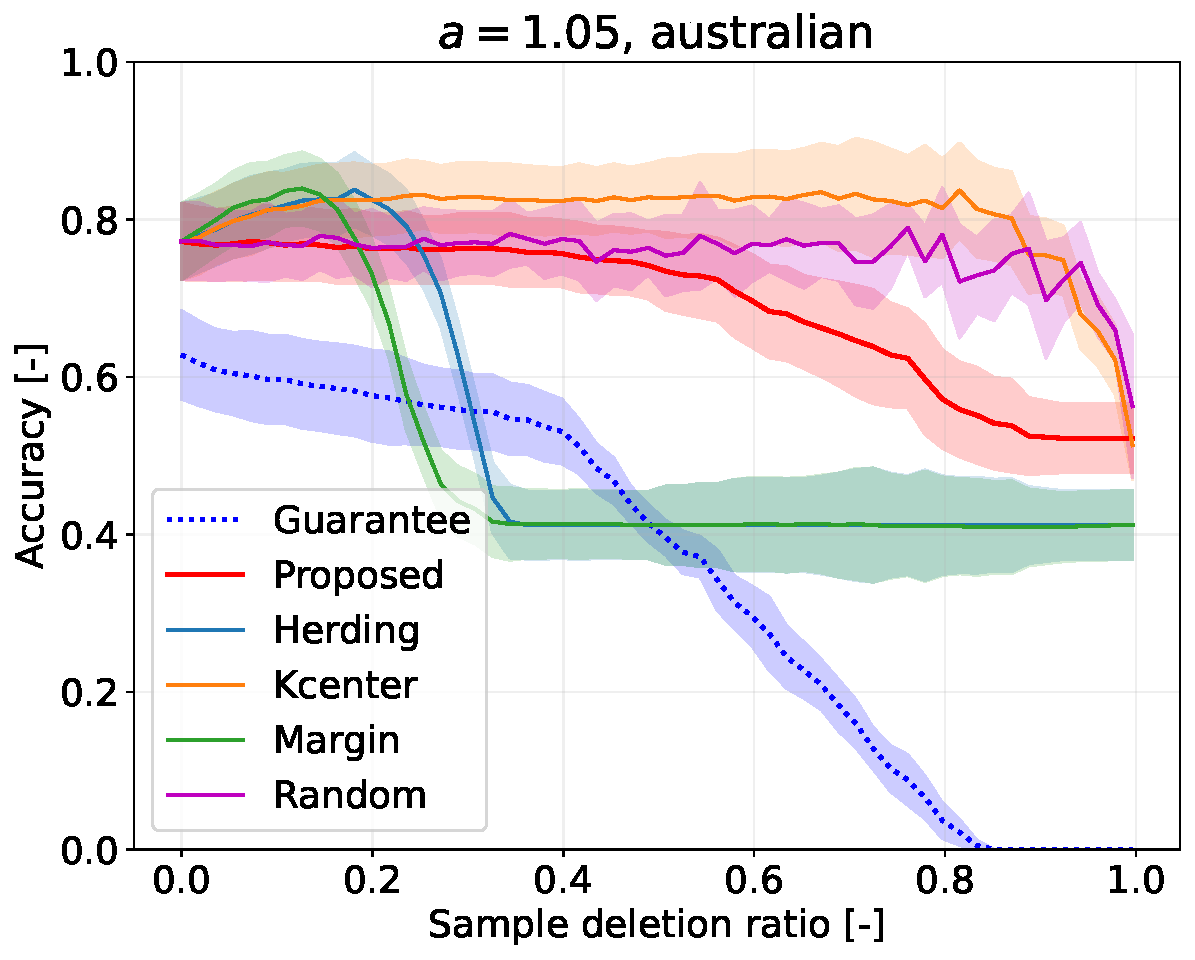
\includegraphics[width=0.8\hsize]{fig/australian/lam_552/a1.05000.pdf}\end{minipage}
	\\
	\begin{minipage}[b]{0.3\hsize}\centering {\small Dataset: breast-cancer, $\lambda=\lambda_\mathrm{best}$}\\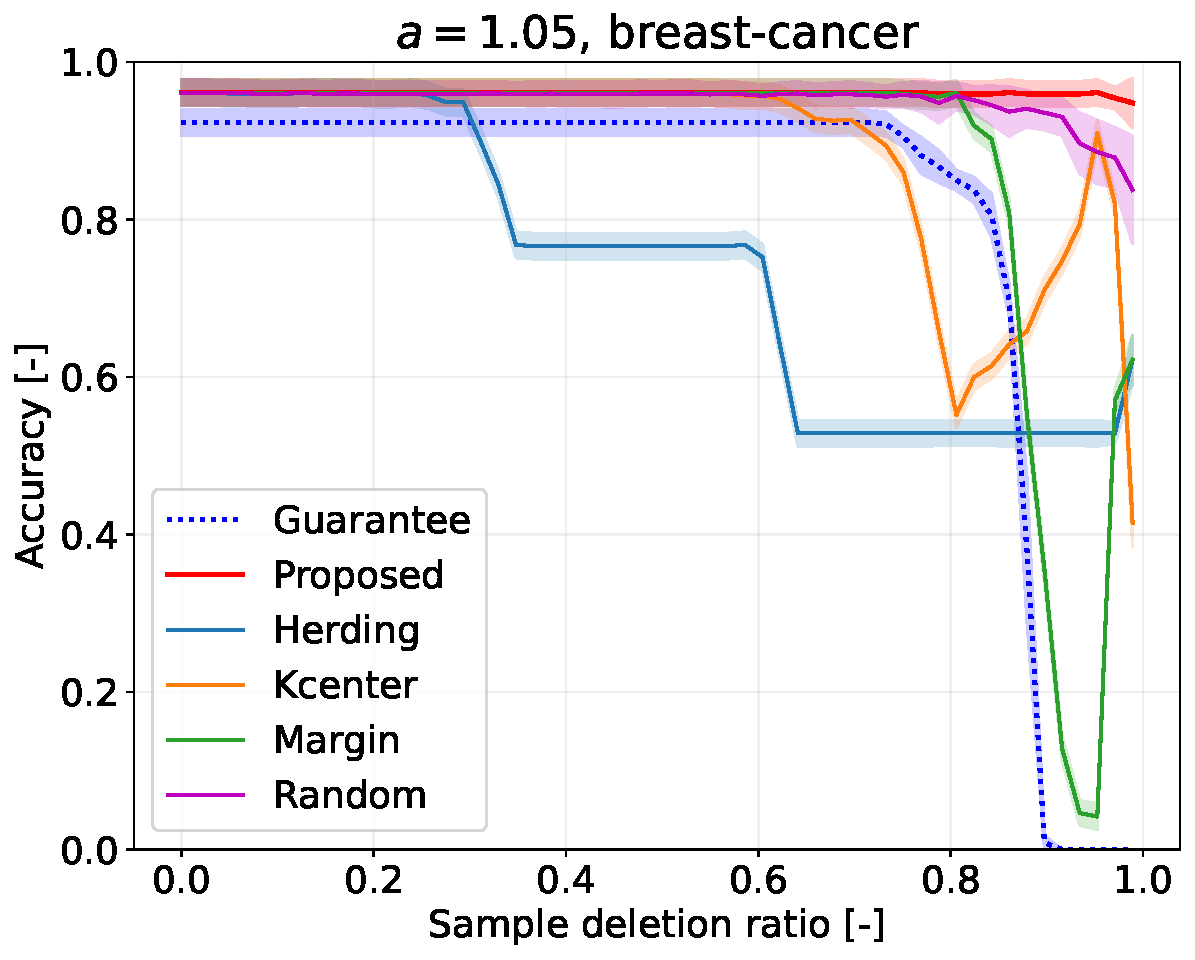
\includegraphics[width=0.8\hsize]{fig/breast/lam_10.0/a1.05000.pdf}\end{minipage}
	&
	\begin{minipage}[b]{0.3\hsize}\centering {\small Dataset: breast-cancer, $\lambda=n \cdot 10^{-1.5}$}\\\includegraphics[width=0.8\hsize]{fig/breast/lam_17.26/a1.05000.pdf}\end{minipage}
	&
	\begin{minipage}[b]{0.3\hsize}\centering {\small Dataset: breast-cancer, $\lambda=n$}\\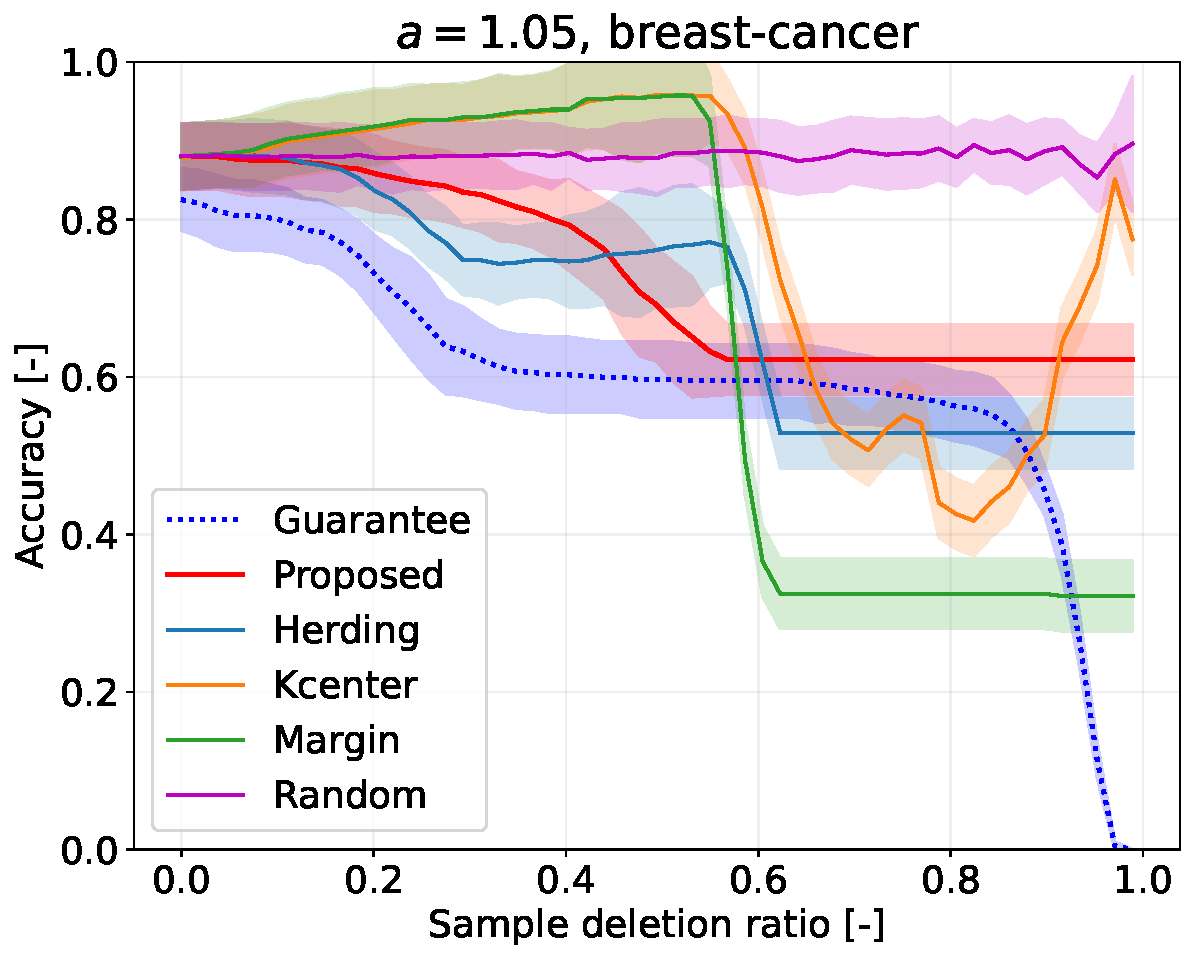
\includegraphics[width=0.8\hsize]{fig/breast/lam_546/a1.05000.pdf}\end{minipage}
	\\
	\begin{minipage}[b]{0.3\hsize}\centering {\small Dataset: heart, $\lambda=\lambda_\mathrm{best}$}\\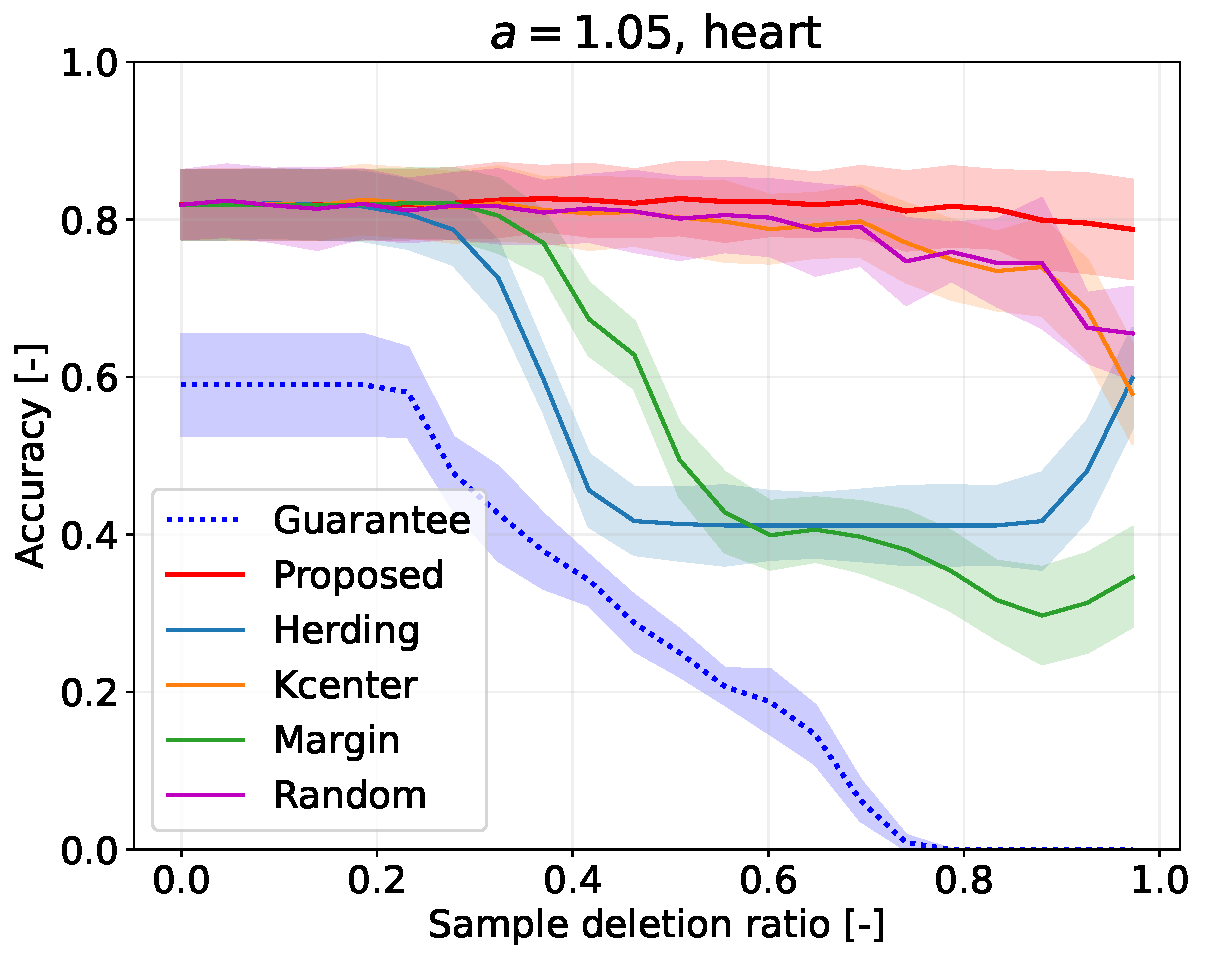
\includegraphics[width=0.8\hsize]{fig/heart/lam_7.0/a1.05000.pdf}\end{minipage}
	&
	\begin{minipage}[b]{0.3\hsize}\centering {\small Dataset: heart, $\lambda=n \cdot 10^{-1.5}$}\\\includegraphics[width=0.8\hsize]{fig/heart/lam_6.830/a1.05000.pdf}\end{minipage}
	&
	\begin{minipage}[b]{0.3\hsize}\centering {\small Dataset: heart, $\lambda=n$}\\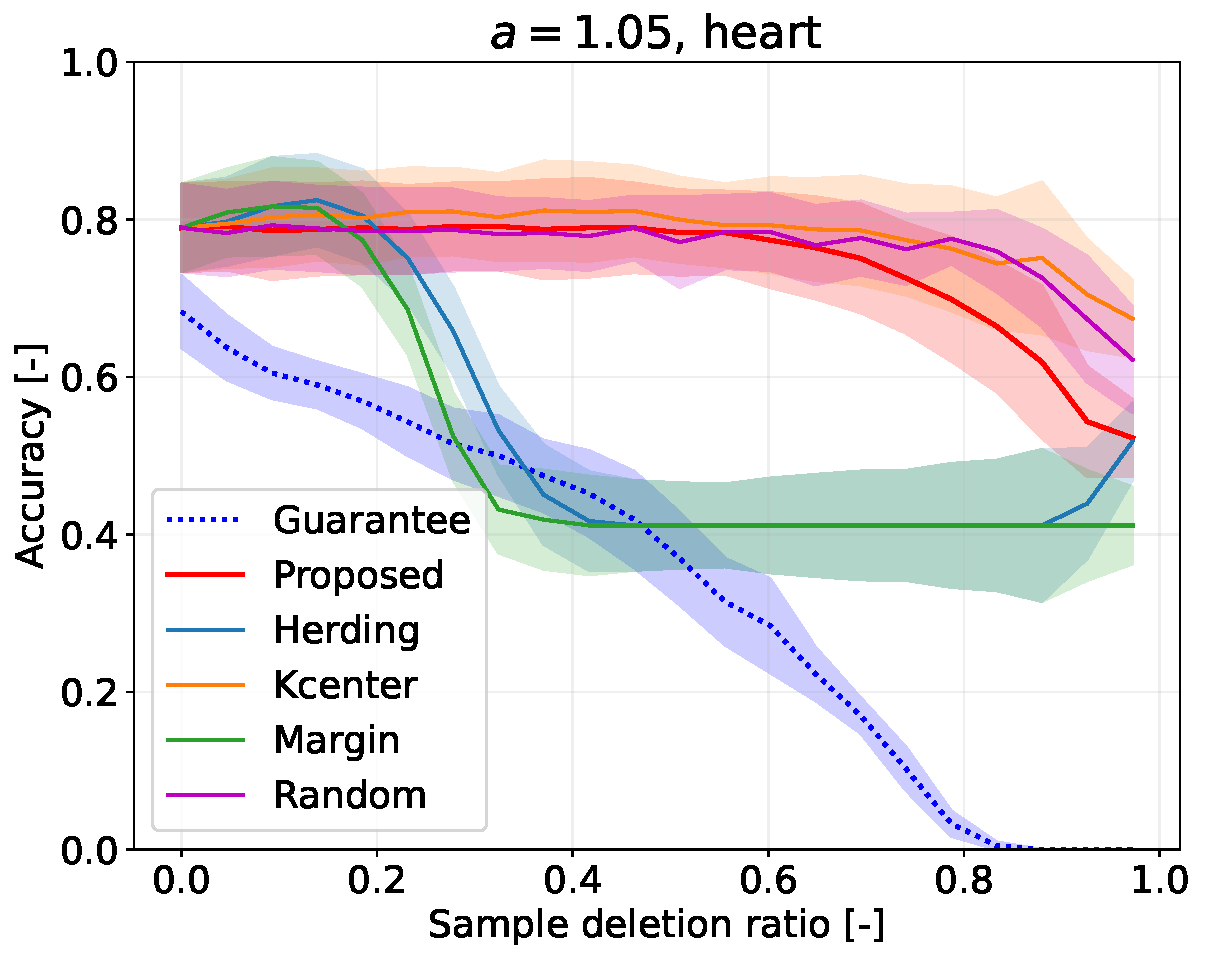
\includegraphics[width=0.8\hsize]{fig/heart/lam_216/a1.05000.pdf}\end{minipage}
	\\
	\begin{minipage}[b]{0.3\hsize}\centering {\small Dataset: ionosphere, $\lambda=\lambda_\mathrm{best}$}\\\includegraphics[width=0.8\hsize]{fig/ionosphere/lam_2.8/a1.05000.pdf}\end{minipage}
	&
	\begin{minipage}[b]{0.3\hsize}\centering {\small Dataset: ionosphere, $\lambda=n \cdot 10^{-1.5}$}\\\includegraphics[width=0.8\hsize]{fig/ionosphere/lam_8.854/a1.05000.pdf}\end{minipage}
	&
	\begin{minipage}[b]{0.3\hsize}\centering {\small Dataset: ionosphere, $\lambda=n$}\\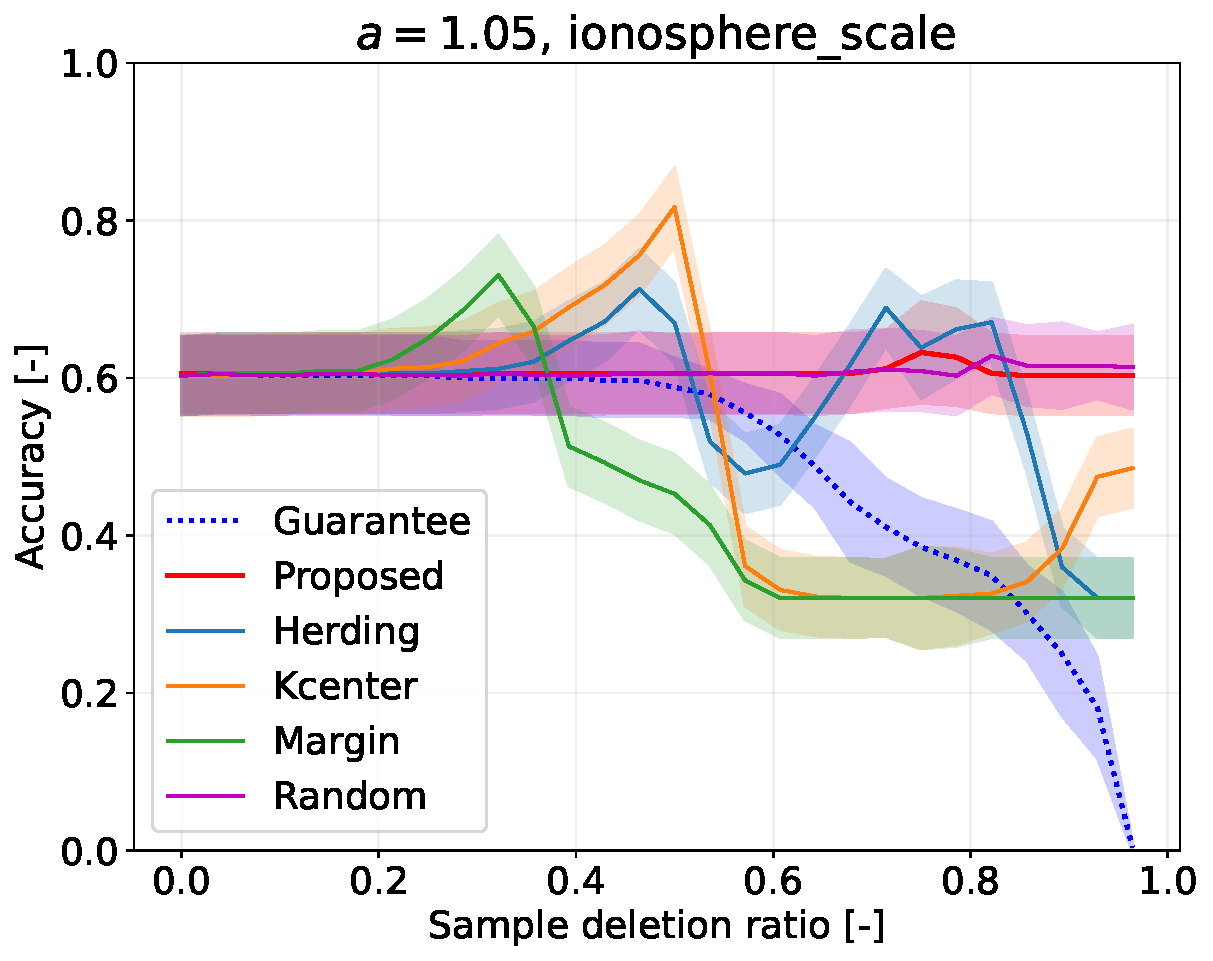
\includegraphics[width=0.8\hsize]{fig/ionosphere/lam_280/a1.05000.pdf}\end{minipage}
	\\
	\begin{minipage}[b]{0.3\hsize}\centering {\small Dataset: splice, $\lambda=\lambda_\mathrm{best}$}\\\includegraphics[width=0.8\hsize]{fig/splice/lam_0.32/a1.05000.pdf}\end{minipage}
	&
	\begin{minipage}[b]{0.3\hsize}\centering {\small Dataset: splice, $\lambda=n_\mathrm \cdot 10^{-1.5}$}\\\includegraphics[width=0.8\hsize]{fig/splice/lam_25.29/a1.05000.pdf}\end{minipage}
	&
	\begin{minipage}[b]{0.3\hsize}\centering {\small Dataset: splice, $\lambda=n$}\\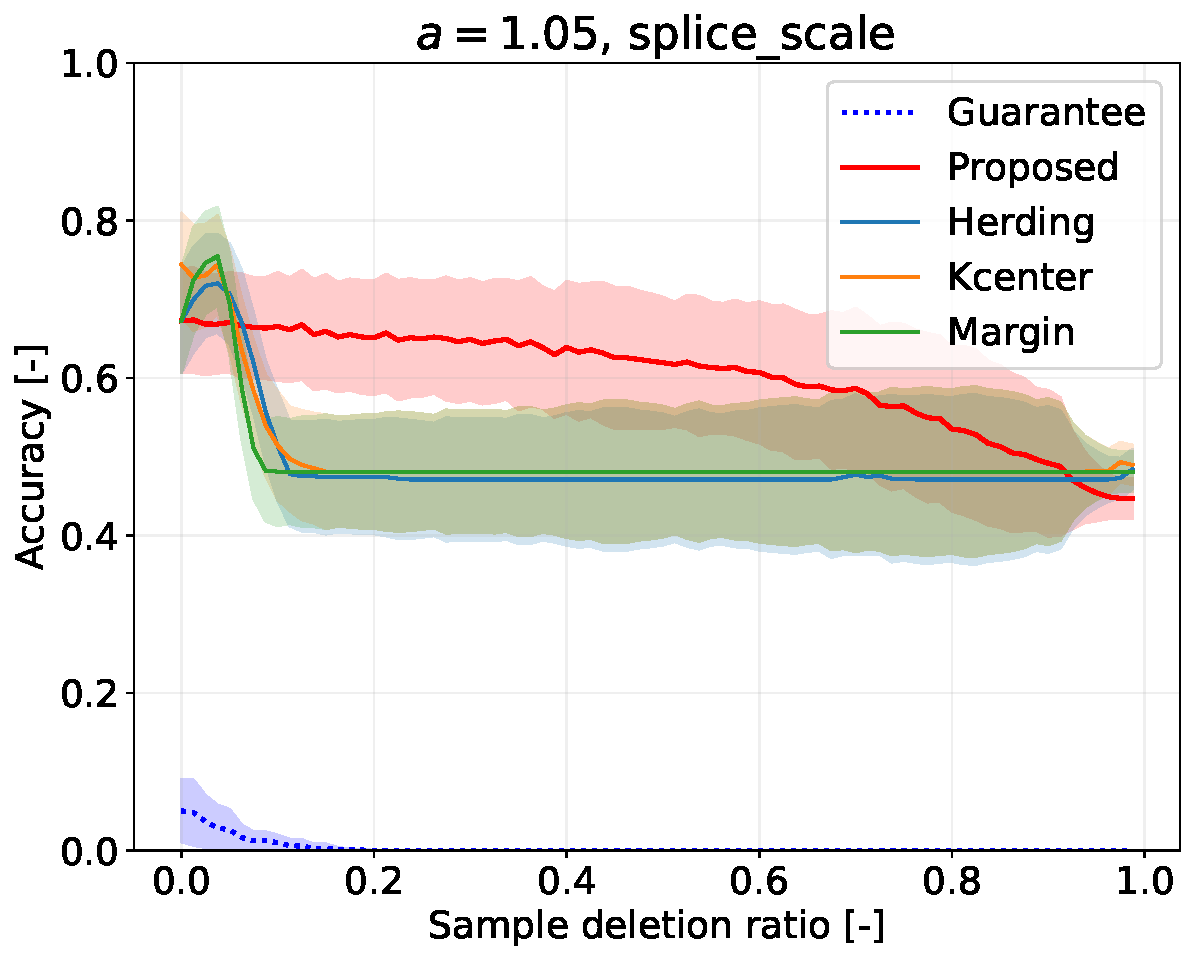
\includegraphics[width=0.8\hsize]{fig/splice/lam_800/a1.05000.pdf}\end{minipage}
	\\

\end{tabular}
\caption{Model performance for RBF-kernel SVMs, under the settings described in Section \ref{sec:experiment} and Appendix \ref{app:experimental-setup}.}
\label{fig:result-acc-svm}
\end{figure}

Next, we show a guarantee of model performance.


\begin{figure}[H]
	\begin{tabular}{ccc}
		\begin{minipage}[b]{0.3\hsize}\centering {\small Dataset: australian, $\lambda=n \cdot 10^{-3}$}\\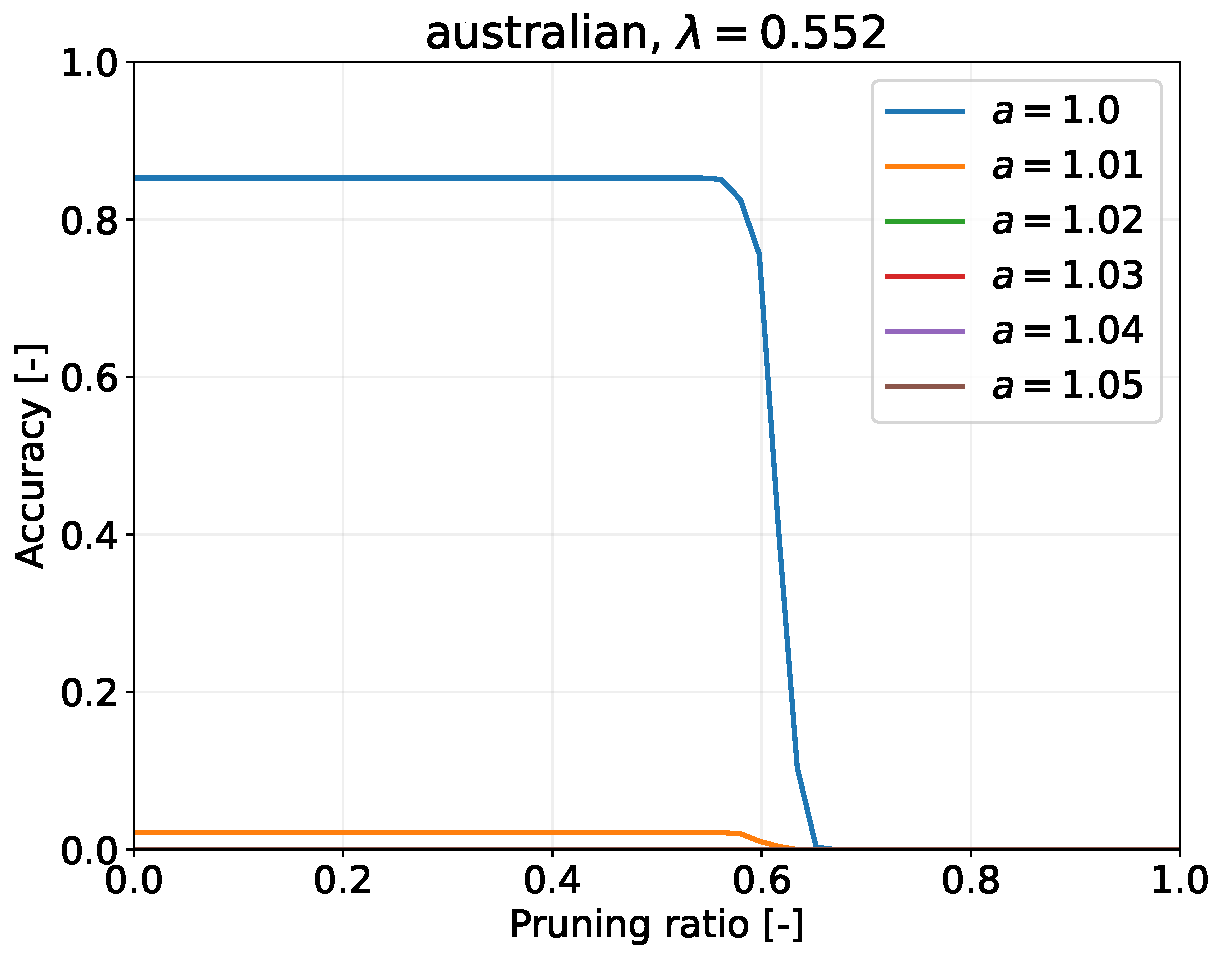
\includegraphics[width=0.8\hsize]{fig/australian/kernel_ss_screening_rate_lam0.552_x_n_y_etest.pdf}\end{minipage}
		&
		\begin{minipage}[b]{0.3\hsize}\centering {\small Dataset: australian, $\lambda=n \cdot 10^{-1.5}$}\\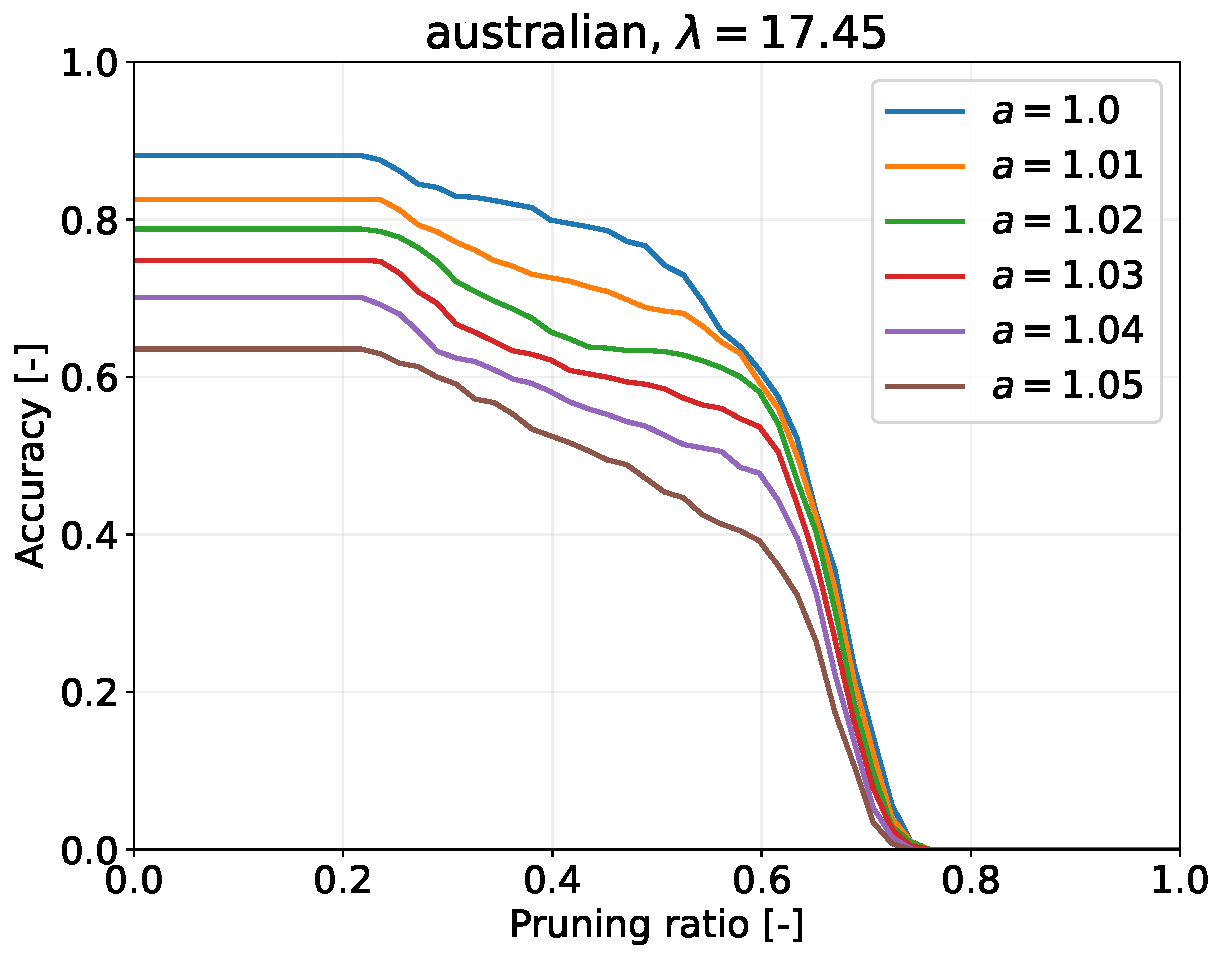
\includegraphics[width=0.8\hsize]{fig/australian/kernel_ss_screening_rate_lam17.45_x_n_y_etest.pdf}\end{minipage}
		&
		\begin{minipage}[b]{0.3\hsize}\centering {\small Dataset: australian, $\lambda=n$}\\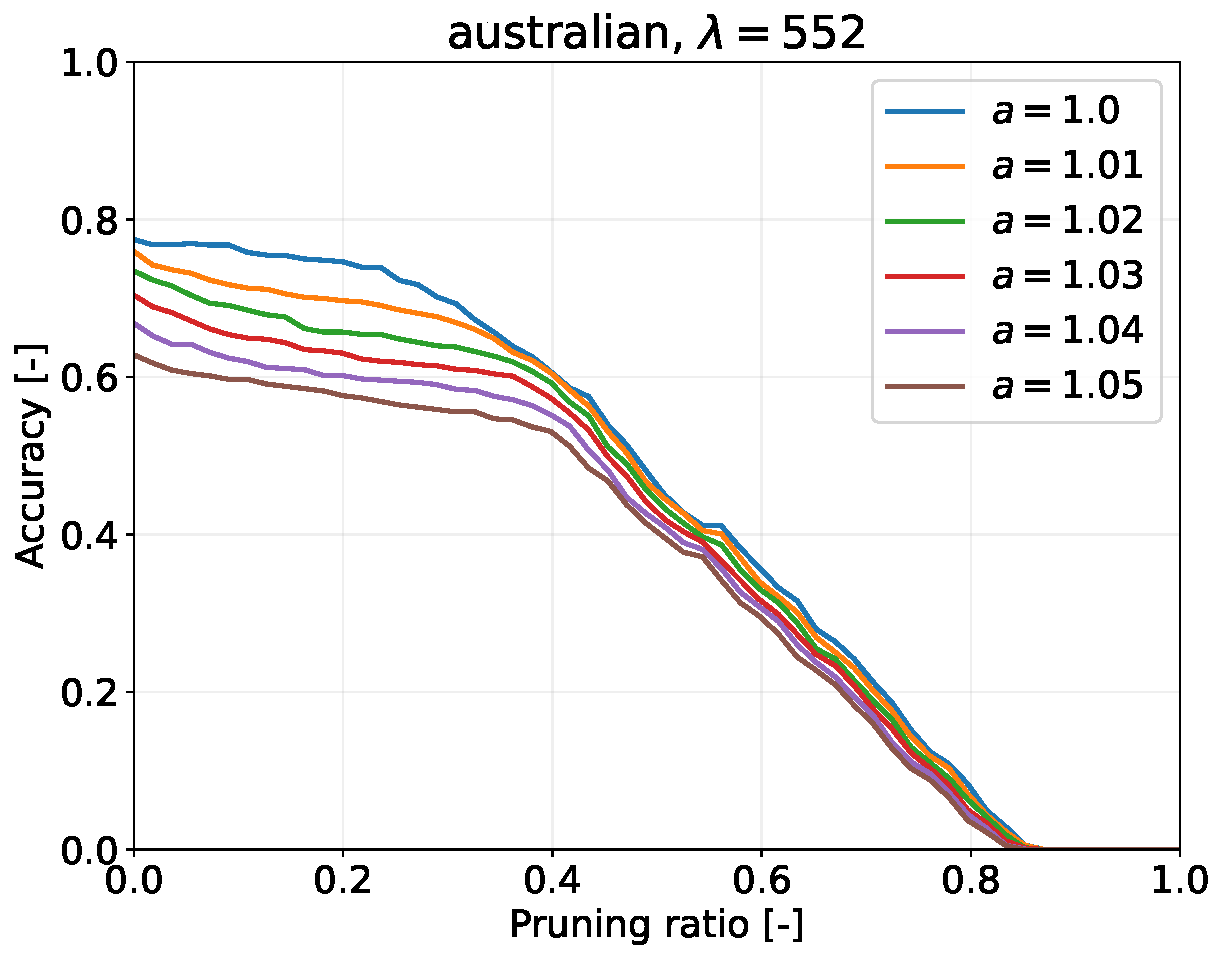
\includegraphics[width=0.8\hsize]{fig/australian/kernel_ss_screening_rate_lam552_x_n_y_etest.pdf}\end{minipage}
		\\
		\begin{minipage}[b]{0.3\hsize}\centering {\small Dataset: breast-cancer, $\lambda=n \cdot 10^{-3}$}\\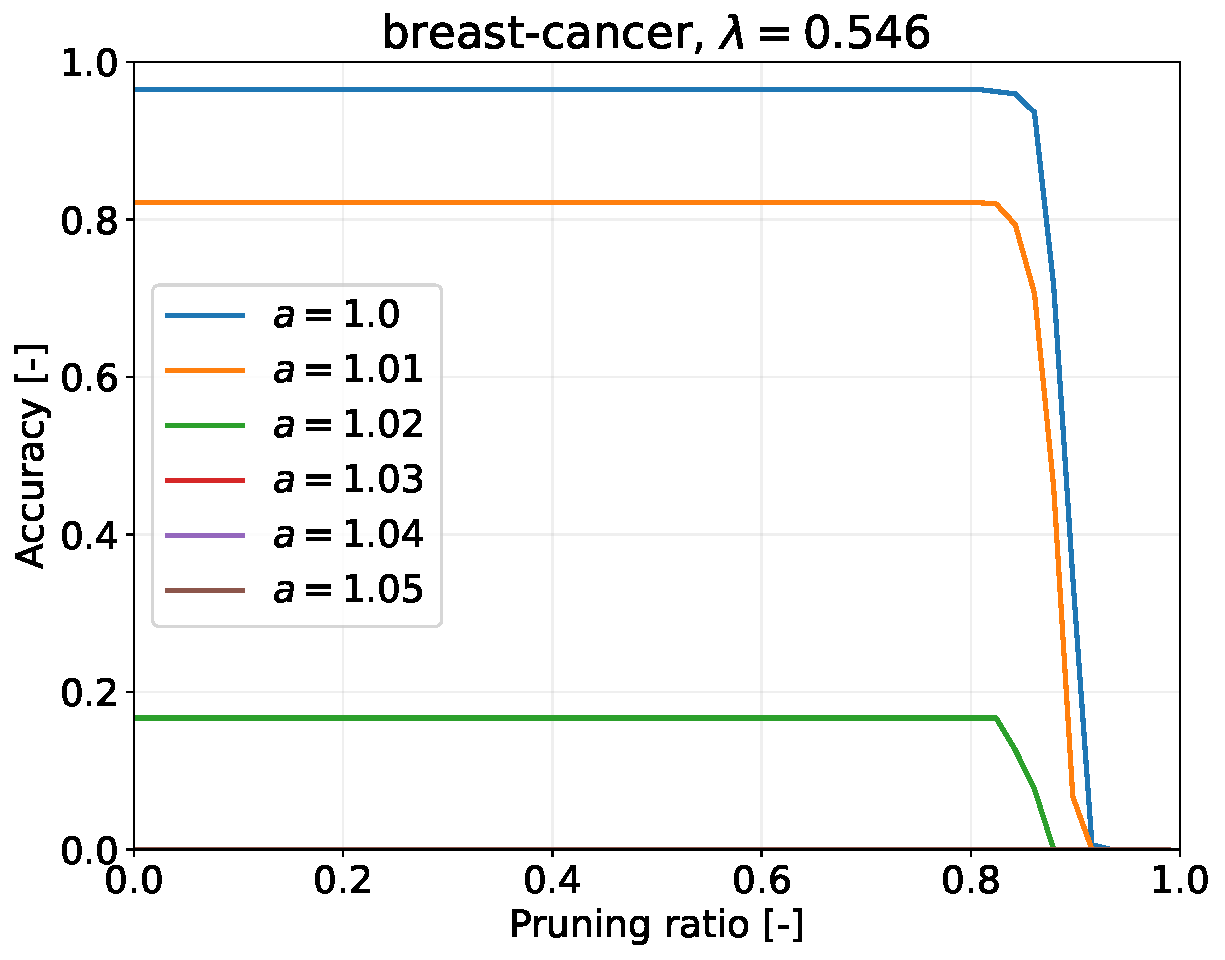
\includegraphics[width=0.8\hsize]{fig/breast/kernel_ss_screening_rate_lam0.546_x_n_y_etest.pdf}\end{minipage}
		&
		\begin{minipage}[b]{0.3\hsize}\centering {\small Dataset: breast-cancer, $\lambda=n \cdot 10^{-1.5}$}\\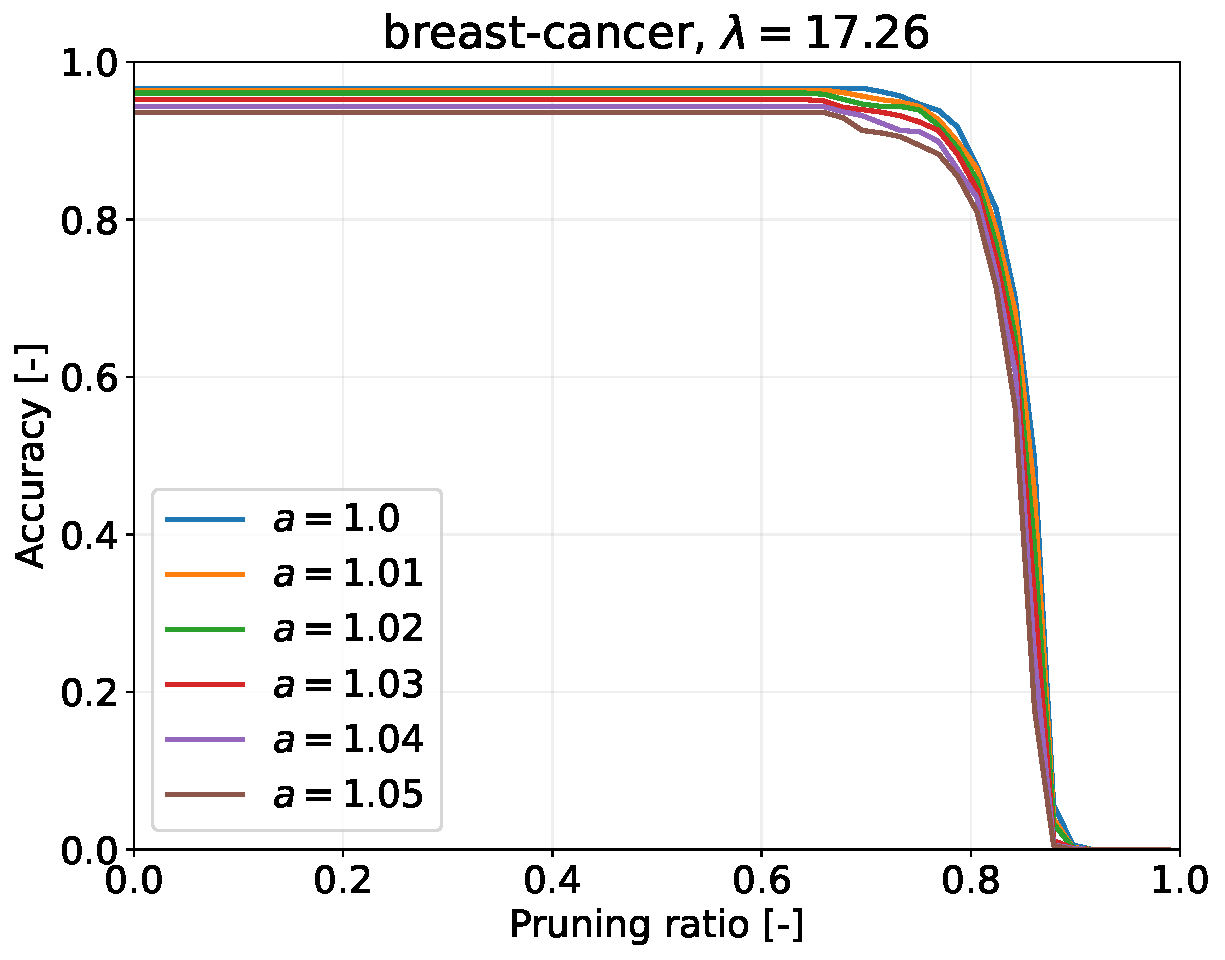
\includegraphics[width=0.8\hsize]{fig/breast/kernel_ss_screening_rate_lam17.26_x_n_y_etest.pdf}\end{minipage}
		&
		\begin{minipage}[b]{0.3\hsize}\centering {\small Dataset: breast-cancer, $\lambda=n$}\\\includegraphics[width=0.8\hsize]{fig/breast/kernel_ss_screening_rate_lam546_x_n_y_etest.pdf}\end{minipage}
		\\
		\begin{minipage}[b]{0.3\hsize}\centering {\small Dataset: heart, $\lambda=n \cdot 10^{-3}$}\\\includegraphics[width=0.8\hsize]{fig/heart/kernel_ss_screening_rate_lam0.216_x_n_y_etest.pdf}\end{minipage}
		&
		\begin{minipage}[b]{0.3\hsize}\centering {\small Dataset: heart, $\lambda=n \cdot 10^{-1.5}$}\\\includegraphics[width=0.8\hsize]{fig/heart/kernel_ss_screening_rate_lam6.830_x_n_y_etest.pdf}\end{minipage}
		&
		\begin{minipage}[b]{0.3\hsize}\centering {\small Dataset: heart, $\lambda=n$}\\\includegraphics[width=0.8\hsize]{fig/heart/kernel_ss_screening_rate_lam216_x_n_y_etest.pdf}\end{minipage}
		\\
		\begin{minipage}[b]{0.3\hsize}\centering {\small Dataset: ionosphere, $\lambda=n \cdot 10^{-3}$}\\\includegraphics[width=0.8\hsize]{fig/ionosphere/kernel_ss_screening_rate_lam0.28_x_n_y_etest.pdf}\end{minipage}
		&
		\begin{minipage}[b]{0.3\hsize}\centering {\small Dataset: ionosphere, $\lambda=n \cdot 10^{-1.5}$}\\\includegraphics[width=0.8\hsize]{fig/ionosphere/kernel_ss_screening_rate_lam8.854_x_n_y_etest.pdf}\end{minipage}
		&
		\begin{minipage}[b]{0.3\hsize}\centering {\small Dataset: ionosphere, $\lambda=n$}\\\includegraphics[width=0.8\hsize]{fig/ionosphere/kernel_ss_screening_rate_lam280_x_n_y_etest.pdf}\end{minipage}
		\\
		\begin{minipage}[b]{0.3\hsize}\centering {\small Dataset: splice, $\lambda=n \cdot 10^{-3}$}\\\includegraphics[width=0.8\hsize]{fig/splice/kernel_ss_screening_rate_lam0.32_x_n_y_etest.pdf}\end{minipage}
		&
		\begin{minipage}[b]{0.3\hsize}\centering {\small Dataset: splice, $\lambda=n_\mathrm \cdot 10^{-1.5}$}\\\includegraphics[width=0.8\hsize]{fig/splice/kernel_ss_screening_rate_lam25.29_x_n_y_etest.pdf}\end{minipage}
		&
		\begin{minipage}[b]{0.3\hsize}\centering {\small Dataset: splice, $\lambda=n$}\\\includegraphics[width=0.8\hsize]{fig/splice/kernel_ss_screening_rate_lam800_x_n_y_etest.pdf}\end{minipage}
		\\
	
	\end{tabular}
	\caption{Model performance for RBF-kernel SVMs, under the settings described in Section \ref{sec:experiment} and Appendix \ref{app:experimental-setup}.}
	\label{fig:result-guarantee-svm}
	\end{figure}

	\newpage

% % % % % % % % % % % % % % % % % % % % % % % % % % % % % %
\subsection{The effectiveness of the proposed method in different models} \label{app:model-disucussion}
% % % % % % % % % % % % % % % % % % % % % % % % % % % % % %

Here, we compare the results between logistic regression in Appendix~\ref{app:result-logistic} and SVM in Appendix~\ref{app:result-svm}.
%
Regarding model performance, there is no significant difference between the two models, and the trends when regularization is large or small are generally consistent for both (Figure~\ref{fig:result-acc-logistic} and \ref{fig:result-acc-svm}).
%
On the other hand, in terms of theoretical evaluation, there are significant differences between the two models (Figure~\ref{fig:result-guarantee-logistic} and \ref{fig:result-guarantee-svm}).
%
The major difference between SVM and logistic regression lies in whether the model is instance-sparse.
%
In SVM, training instances where \(\alpha^*_{\bm 1_n, \bm 1_n, i} = 0\) do not affect the duality gap during instance selection.
%
Therefore, more effective instance selection is possible, as the duality gap can be suppressed further.
%
In contrast, logistic regression is not a sparse model, and as a result, the theoretical lower bound of the worst-case weighted validation accuracy is expected to be lower than that of SVM.

% % % % % % % % % % % % % % % % % % % % % % % % % % % % % %
\subsection{Experimental Results Using NTK in Section \ref{subsec:result-image}} \label{app:result-ntk}
% % % % % % % % % % % % % % % % % % % % % % % % % % % % % %

%
We also experimented the DRCS method with NTK for an image dataset.
%
We composed 5,000-sample binary classification dataset from “CIFAR-10” dataset by choosing from classes “airplane” and "automobile”.
%
A total of 1000 instances were sampled, and experiments were conducted using Algorithm~\ref{alg:1}.
%
It was demonstrated that the proposed DRCS method could be approximately applied to deep learning by using NTK.
%
\begin{figure}[H]
\begin{tabular}{ccc}
\begin{minipage}[b]{0.3\hsize}\centering {\small Dataset: CIFAR10, $\lambda=n \cdot 10^{-3}$}\\\includegraphics[width=0.8\hsize]{fig/table_logistic/cifar10-logistic/cntk/lam_1_/a1.05000.pdf}\end{minipage}
&
\begin{minipage}[b]{0.3\hsize}\centering {\small Dataset: CIFAR10, $\lambda=n \cdot 10^{-1.5}$}\\\includegraphics[width=0.8\hsize]{fig/table_logistic/cifar10-logistic/cntk/lam_31.62/a1.05000.pdf}\end{minipage}
&
\begin{minipage}[b]{0.3\hsize}\centering {\small Dataset: CIFAR10, $\lambda=n$}\\\includegraphics[width=0.8\hsize]{fig/table_logistic/cifar10-logistic/cntk/lam_1000/a1.05000.pdf}\end{minipage}
\\
\begin{minipage}[b]{0.3\hsize}\centering {\small Dataset: CIFAR10, $\lambda=n \cdot 10^{-3}$}\\\includegraphics[width=0.8\hsize]{fig/table_logistic/cifar10-logistic/cntk/cntk_ss_screening_rate_lam1._x_n_y_etest.pdf}\end{minipage}
&
\begin{minipage}[b]{0.3\hsize}\centering {\small Dataset: CIFAR10, $\lambda=n \cdot 10^{-1.5}$}\\\includegraphics[width=0.8\hsize]{fig/table_logistic/cifar10-logistic/cntk/cntk_ss_screening_rate_lam31.62_x_n_y_etest.pdf}\end{minipage}
&
\begin{minipage}[b]{0.3\hsize}\centering {\small Dataset: CIFAR10, $\lambda=n$}\\\includegraphics[width=0.8\hsize]{fig/table_logistic/cifar10-logistic/cntk/cntk_ss_screening_rate_lam1000_x_n_y_etest.pdf}\end{minipage}

\end{tabular}
\caption{Model performance for NTK, under the settings described in Section \ref{sec:experiment} and Appendix \ref{app:experimental-setup}.}
\label{fig:result-ntk-acc}
\end{figure}